% Options for packages loaded elsewhere
\PassOptionsToPackage{unicode}{hyperref}
\PassOptionsToPackage{hyphens}{url}
%
\documentclass[
]{article}
\usepackage{amsmath,amssymb}
\usepackage{iftex}
\ifPDFTeX
  \usepackage[T1]{fontenc}
  \usepackage[utf8]{inputenc}
  \usepackage{textcomp} % provide euro and other symbols
\else % if luatex or xetex
  \usepackage{unicode-math} % this also loads fontspec
  \defaultfontfeatures{Scale=MatchLowercase}
  \defaultfontfeatures[\rmfamily]{Ligatures=TeX,Scale=1}
\fi
\usepackage{lmodern}
\ifPDFTeX\else
  % xetex/luatex font selection
  \setmainfont[]{Roboto}
  \setmonofont[]{Consolas}
\fi
% Use upquote if available, for straight quotes in verbatim environments
\IfFileExists{upquote.sty}{\usepackage{upquote}}{}
\IfFileExists{microtype.sty}{% use microtype if available
  \usepackage[]{microtype}
  \UseMicrotypeSet[protrusion]{basicmath} % disable protrusion for tt fonts
}{}
\makeatletter
\@ifundefined{KOMAClassName}{% if non-KOMA class
  \IfFileExists{parskip.sty}{%
    \usepackage{parskip}
  }{% else
    \setlength{\parindent}{0pt}
    \setlength{\parskip}{6pt plus 2pt minus 1pt}}
}{% if KOMA class
  \KOMAoptions{parskip=half}}
\makeatother
\usepackage{xcolor}
\usepackage[margin=1in]{geometry}
\usepackage{color}
\usepackage{fancyvrb}
\newcommand{\VerbBar}{|}
\newcommand{\VERB}{\Verb[commandchars=\\\{\}]}
\DefineVerbatimEnvironment{Highlighting}{Verbatim}{commandchars=\\\{\}}
% Add ',fontsize=\small' for more characters per line
\usepackage{framed}
\definecolor{shadecolor}{RGB}{248,248,248}
\newenvironment{Shaded}{\begin{snugshade}}{\end{snugshade}}
\newcommand{\AlertTok}[1]{\textcolor[rgb]{0.94,0.16,0.16}{#1}}
\newcommand{\AnnotationTok}[1]{\textcolor[rgb]{0.56,0.35,0.01}{\textbf{\textit{#1}}}}
\newcommand{\AttributeTok}[1]{\textcolor[rgb]{0.13,0.29,0.53}{#1}}
\newcommand{\BaseNTok}[1]{\textcolor[rgb]{0.00,0.00,0.81}{#1}}
\newcommand{\BuiltInTok}[1]{#1}
\newcommand{\CharTok}[1]{\textcolor[rgb]{0.31,0.60,0.02}{#1}}
\newcommand{\CommentTok}[1]{\textcolor[rgb]{0.56,0.35,0.01}{\textit{#1}}}
\newcommand{\CommentVarTok}[1]{\textcolor[rgb]{0.56,0.35,0.01}{\textbf{\textit{#1}}}}
\newcommand{\ConstantTok}[1]{\textcolor[rgb]{0.56,0.35,0.01}{#1}}
\newcommand{\ControlFlowTok}[1]{\textcolor[rgb]{0.13,0.29,0.53}{\textbf{#1}}}
\newcommand{\DataTypeTok}[1]{\textcolor[rgb]{0.13,0.29,0.53}{#1}}
\newcommand{\DecValTok}[1]{\textcolor[rgb]{0.00,0.00,0.81}{#1}}
\newcommand{\DocumentationTok}[1]{\textcolor[rgb]{0.56,0.35,0.01}{\textbf{\textit{#1}}}}
\newcommand{\ErrorTok}[1]{\textcolor[rgb]{0.64,0.00,0.00}{\textbf{#1}}}
\newcommand{\ExtensionTok}[1]{#1}
\newcommand{\FloatTok}[1]{\textcolor[rgb]{0.00,0.00,0.81}{#1}}
\newcommand{\FunctionTok}[1]{\textcolor[rgb]{0.13,0.29,0.53}{\textbf{#1}}}
\newcommand{\ImportTok}[1]{#1}
\newcommand{\InformationTok}[1]{\textcolor[rgb]{0.56,0.35,0.01}{\textbf{\textit{#1}}}}
\newcommand{\KeywordTok}[1]{\textcolor[rgb]{0.13,0.29,0.53}{\textbf{#1}}}
\newcommand{\NormalTok}[1]{#1}
\newcommand{\OperatorTok}[1]{\textcolor[rgb]{0.81,0.36,0.00}{\textbf{#1}}}
\newcommand{\OtherTok}[1]{\textcolor[rgb]{0.56,0.35,0.01}{#1}}
\newcommand{\PreprocessorTok}[1]{\textcolor[rgb]{0.56,0.35,0.01}{\textit{#1}}}
\newcommand{\RegionMarkerTok}[1]{#1}
\newcommand{\SpecialCharTok}[1]{\textcolor[rgb]{0.81,0.36,0.00}{\textbf{#1}}}
\newcommand{\SpecialStringTok}[1]{\textcolor[rgb]{0.31,0.60,0.02}{#1}}
\newcommand{\StringTok}[1]{\textcolor[rgb]{0.31,0.60,0.02}{#1}}
\newcommand{\VariableTok}[1]{\textcolor[rgb]{0.00,0.00,0.00}{#1}}
\newcommand{\VerbatimStringTok}[1]{\textcolor[rgb]{0.31,0.60,0.02}{#1}}
\newcommand{\WarningTok}[1]{\textcolor[rgb]{0.56,0.35,0.01}{\textbf{\textit{#1}}}}
\usepackage{graphicx}
\makeatletter
\def\maxwidth{\ifdim\Gin@nat@width>\linewidth\linewidth\else\Gin@nat@width\fi}
\def\maxheight{\ifdim\Gin@nat@height>\textheight\textheight\else\Gin@nat@height\fi}
\makeatother
% Scale images if necessary, so that they will not overflow the page
% margins by default, and it is still possible to overwrite the defaults
% using explicit options in \includegraphics[width, height, ...]{}
\setkeys{Gin}{width=\maxwidth,height=\maxheight,keepaspectratio}
% Set default figure placement to htbp
\makeatletter
\def\fps@figure{htbp}
\makeatother
\setlength{\emergencystretch}{3em} % prevent overfull lines
\providecommand{\tightlist}{%
  \setlength{\itemsep}{0pt}\setlength{\parskip}{0pt}}
\setcounter{secnumdepth}{-\maxdimen} % remove section numbering
\usepackage{fvextra} \DefineVerbatimEnvironment{Highlighting}{Verbatim}{breaklines,commandchars=\\\{\}}
\ifLuaTeX
  \usepackage{selnolig}  % disable illegal ligatures
\fi
\IfFileExists{bookmark.sty}{\usepackage{bookmark}}{\usepackage{hyperref}}
\IfFileExists{xurl.sty}{\usepackage{xurl}}{} % add URL line breaks if available
\urlstyle{same}
\hypersetup{
  pdftitle={Quantium Virtual Internship - Retail Strategy and Analytics - Task 1},
  hidelinks,
  pdfcreator={LaTeX via pandoc}}

\title{Quantium Virtual Internship - Retail Strategy and Analytics -
Task 1}
\author{}
\date{\vspace{-2.5em}}

\begin{document}
\maketitle

\hypertarget{solution-template-for-task-1}{%
\section{Solution template for Task
1}\label{solution-template-for-task-1}}

This file is a solution template for the Task 1 of the Quantium Virtual
Internship. It will walk you through the analysis, providing the
scaffolding for your solution with gaps left for you to fill in
yourself.

Look for comments that say ``over to you'' for places where you need to
add your own code! Often, there will be hints about what to do or what
function to use in the text leading up to a code block - if you need a
bit of extra help on how to use a function, the internet has many
excellent resources on R coding, which you can find using your favourite
search engine.

\hypertarget{load-required-libraries-and-datasets}{%
\subsection{Load required libraries and
datasets}\label{load-required-libraries-and-datasets}}

Note that you will need to install these libraries if you have never
used these before.

\begin{Shaded}
\begin{Highlighting}[]
\DocumentationTok{\#\#\#\# Example code to install packages}
\CommentTok{\#install.packages("data.table")}
\DocumentationTok{\#\#\#\# Load required libraries}
\FunctionTok{library}\NormalTok{(}\StringTok{"data.table"}\NormalTok{)}
\end{Highlighting}
\end{Shaded}

\begin{verbatim}
## Warning: package 'data.table' was built under R version 4.3.1
\end{verbatim}

\begin{Shaded}
\begin{Highlighting}[]
\FunctionTok{library}\NormalTok{(ggplot2)}
\end{Highlighting}
\end{Shaded}

\begin{verbatim}
## Warning: package 'ggplot2' was built under R version 4.3.1
\end{verbatim}

\begin{Shaded}
\begin{Highlighting}[]
\FunctionTok{library}\NormalTok{(ggmosaic)}
\end{Highlighting}
\end{Shaded}

\begin{verbatim}
## Warning: package 'ggmosaic' was built under R version 4.3.1
\end{verbatim}

\begin{Shaded}
\begin{Highlighting}[]
\FunctionTok{library}\NormalTok{(readr)}
\end{Highlighting}
\end{Shaded}

\begin{verbatim}
## Warning: package 'readr' was built under R version 4.3.1
\end{verbatim}

\begin{Shaded}
\begin{Highlighting}[]
\FunctionTok{library}\NormalTok{(plyr)}
\end{Highlighting}
\end{Shaded}

\begin{verbatim}
## Warning: package 'plyr' was built under R version 4.3.1
\end{verbatim}

\begin{Shaded}
\begin{Highlighting}[]
\FunctionTok{library}\NormalTok{(dplyr)}
\end{Highlighting}
\end{Shaded}

\begin{verbatim}
## Warning: package 'dplyr' was built under R version 4.3.1
\end{verbatim}

\begin{verbatim}
## 
## Attaching package: 'dplyr'
\end{verbatim}

\begin{verbatim}
## The following objects are masked from 'package:plyr':
## 
##     arrange, count, desc, failwith, id, mutate, rename, summarise,
##     summarize
\end{verbatim}

\begin{verbatim}
## The following objects are masked from 'package:data.table':
## 
##     between, first, last
\end{verbatim}

\begin{verbatim}
## The following objects are masked from 'package:stats':
## 
##     filter, lag
\end{verbatim}

\begin{verbatim}
## The following objects are masked from 'package:base':
## 
##     intersect, setdiff, setequal, union
\end{verbatim}

\begin{Shaded}
\begin{Highlighting}[]
\FunctionTok{library}\NormalTok{(lubridate)}
\end{Highlighting}
\end{Shaded}

\begin{verbatim}
## Warning: package 'lubridate' was built under R version 4.2.3
\end{verbatim}

\begin{verbatim}
## 
## Attaching package: 'lubridate'
\end{verbatim}

\begin{verbatim}
## The following objects are masked from 'package:data.table':
## 
##     hour, isoweek, mday, minute, month, quarter, second, wday, week,
##     yday, year
\end{verbatim}

\begin{verbatim}
## The following objects are masked from 'package:base':
## 
##     date, intersect, setdiff, union
\end{verbatim}

\begin{Shaded}
\begin{Highlighting}[]
\FunctionTok{library}\NormalTok{(stringr)}
\end{Highlighting}
\end{Shaded}

\begin{verbatim}
## Warning: package 'stringr' was built under R version 4.3.1
\end{verbatim}

\begin{Shaded}
\begin{Highlighting}[]
\FunctionTok{library}\NormalTok{(arules)}
\end{Highlighting}
\end{Shaded}

\begin{verbatim}
## Warning: package 'arules' was built under R version 4.2.3
\end{verbatim}

\begin{verbatim}
## Loading required package: Matrix
\end{verbatim}

\begin{verbatim}
## 
## Attaching package: 'arules'
\end{verbatim}

\begin{verbatim}
## The following object is masked from 'package:dplyr':
## 
##     recode
\end{verbatim}

\begin{verbatim}
## The following objects are masked from 'package:base':
## 
##     abbreviate, write
\end{verbatim}

\begin{Shaded}
\begin{Highlighting}[]
\FunctionTok{library}\NormalTok{(arulesViz)}
\end{Highlighting}
\end{Shaded}

\begin{verbatim}
## Warning: package 'arulesViz' was built under R version 4.2.3
\end{verbatim}

\begin{Shaded}
\begin{Highlighting}[]
\DocumentationTok{\#\#\#\# Point the filePath to where you have downloaded the datasets to and }
\DocumentationTok{\#\#\#\# assign the data files to data.tables}
\CommentTok{\# over to you! fill in the path to your working directory. If you are on a Windows machine, you will need to use forward slashes (/) instead of backshashes (\textbackslash{})}
\NormalTok{filePath }\OtherTok{\textless{}{-}} \FunctionTok{paste0}\NormalTok{(}\FunctionTok{getwd}\NormalTok{(),}\StringTok{"/"}\NormalTok{)}
\NormalTok{transactionData }\OtherTok{\textless{}{-}} \FunctionTok{fread}\NormalTok{(}\AttributeTok{file =} \FunctionTok{paste0}\NormalTok{(filePath,}\StringTok{"QVI\_transaction\_data.xlsx {-} in.csv"}\NormalTok{), }\AttributeTok{header =} \ConstantTok{TRUE}\NormalTok{)}
\NormalTok{customerData }\OtherTok{\textless{}{-}} \FunctionTok{fread}\NormalTok{(}\AttributeTok{file =} \FunctionTok{paste0}\NormalTok{(filePath,}\StringTok{"QVI\_purchase\_behaviour.csv"}\NormalTok{), }\AttributeTok{header =} \ConstantTok{TRUE}\NormalTok{)}
\end{Highlighting}
\end{Shaded}

\hypertarget{exploratory-data-analysis}{%
\subsection{Exploratory data analysis}\label{exploratory-data-analysis}}

The first step in any analysis is to first understand the data. Let's
take a look at each of the datasets provided. \#\#\# Examining
transaction data We can use \texttt{str()} to look at the format of each
column and see a sample of the data. As we have read in the dataset as a
\texttt{data.table} object, we can also run \texttt{transactionData} in
the console to see a sample of the data or use
\texttt{head(transactionData)} to look at the first 10 rows. Let's check
if columns we would expect to be numeric are in numeric form and date
columns are in date format.

\begin{Shaded}
\begin{Highlighting}[]
\DocumentationTok{\#\#\#\# Examine transaction data}
\CommentTok{\# Over to you! Examine the data using one or more of the methods described above.}

\FunctionTok{str}\NormalTok{(transactionData)}
\end{Highlighting}
\end{Shaded}

\begin{verbatim}
## Classes 'data.table' and 'data.frame': 264836 obs. of 8 variables:
## $ DATE : int 43390 43599 43605 43329 43330 43604 43601 43601 43332 43330 ...
## $ STORE_NBR : int 1 1 1 2 2 4 4 4 5 7 ...
## $ LYLTY_CARD_NBR: int 1000 1307 1343 2373 2426 4074 4149 4196 5026 7150 ...
## $ TXN_ID : int 1 348 383 974 1038 2982 3333 3539 4525 6900 ...
## $ PROD_NBR : int 5 66 61 69 108 57 16 24 42 52 ...
## $ PROD_NAME : chr "Natural Chip Compny SeaSalt175g" "CCs Nacho Cheese 175g"
"Smiths Crinkle Cut Chips Chicken 170g" "Smiths Chip Thinly S/Cream&Onion 175g"
...
## $ PROD_QTY : int 2 3 2 5 3 1 1 1 1 2 ...
## $ TOT_SALES : num 6 6.3 2.9 15 13.8 5.1 5.7 3.6 3.9 7.2 ...
## - attr(*, ".internal.selfref")=<externalptr>
\end{verbatim}

\begin{Shaded}
\begin{Highlighting}[]
\NormalTok{transactionData}
\end{Highlighting}
\end{Shaded}

\begin{verbatim}
##          DATE STORE_NBR LYLTY_CARD_NBR TXN_ID PROD_NBR
##      1: 43390         1           1000      1        5
##      2: 43599         1           1307    348       66
##      3: 43605         1           1343    383       61
##      4: 43329         2           2373    974       69
##      5: 43330         2           2426   1038      108
##     ---                                               
## 264832: 43533       272         272319 270088       89
## 264833: 43325       272         272358 270154       74
## 264834: 43410       272         272379 270187       51
## 264835: 43461       272         272379 270188       42
## 264836: 43365       272         272380 270189       74
##                                        PROD_NAME PROD_QTY TOT_SALES
##      1:   Natural Chip        Compny SeaSalt175g        2       6.0
##      2:                 CCs Nacho Cheese    175g        3       6.3
##      3:   Smiths Crinkle Cut  Chips Chicken 170g        2       2.9
##      4:   Smiths Chip Thinly  S/Cream&Onion 175g        5      15.0
##      5: Kettle Tortilla ChpsHny&Jlpno Chili 150g        3      13.8
##     ---                                                            
## 264832:  Kettle Sweet Chilli And Sour Cream 175g        2      10.8
## 264833:            Tostitos Splash Of  Lime 175g        1       4.4
## 264834:                 Doritos Mexicana    170g        2       8.8
## 264835:  Doritos Corn Chip Mexican Jalapeno 150g        2       7.8
## 264836:            Tostitos Splash Of  Lime 175g        2       8.8
\end{verbatim}

We can see that the date column is in an integer format. Let's change
this to a date format.

\begin{Shaded}
\begin{Highlighting}[]
\DocumentationTok{\#\#\#\# Convert DATE column to a date format}
\DocumentationTok{\#\#\#\# A quick search online tells us that CSV and Excel integer dates begin on 30 Dec 1899}

\NormalTok{transactionData}\SpecialCharTok{$}\NormalTok{DATE }\OtherTok{\textless{}{-}} \FunctionTok{as.Date}\NormalTok{(transactionData}\SpecialCharTok{$}\NormalTok{DATE, }\AttributeTok{origin =} \StringTok{"1899{-}12{-}30"}\NormalTok{)}
\end{Highlighting}
\end{Shaded}

We should check that we are looking at the right products by examining
PROD\_NAME.

\begin{Shaded}
\begin{Highlighting}[]
\DocumentationTok{\#\#\#\# Examine PROD\_NAME}
\CommentTok{\# Over to you! Generate a summary of the PROD\_NAME column.}

\NormalTok{transactionData}\SpecialCharTok{$}\NormalTok{PROD\_NAME[}\DecValTok{1}\SpecialCharTok{:}\DecValTok{10}\NormalTok{]}
\end{Highlighting}
\end{Shaded}

\begin{verbatim}
##  [1] "Natural Chip        Compny SeaSalt175g"  
##  [2] "CCs Nacho Cheese    175g"                
##  [3] "Smiths Crinkle Cut  Chips Chicken 170g"  
##  [4] "Smiths Chip Thinly  S/Cream&Onion 175g"  
##  [5] "Kettle Tortilla ChpsHny&Jlpno Chili 150g"
##  [6] "Old El Paso Salsa   Dip Tomato Mild 300g"
##  [7] "Smiths Crinkle Chips Salt & Vinegar 330g"
##  [8] "Grain Waves         Sweet Chilli 210g"   
##  [9] "Doritos Corn Chip Mexican Jalapeno 150g" 
## [10] "Grain Waves Sour    Cream&Chives 210G"
\end{verbatim}

\begin{Shaded}
\begin{Highlighting}[]
\FunctionTok{summary}\NormalTok{(transactionData}\SpecialCharTok{$}\NormalTok{PROD\_NAME)}
\end{Highlighting}
\end{Shaded}

\begin{verbatim}
##    Length     Class      Mode 
##    264836 character character
\end{verbatim}

Looks like we are definitely looking at potato chips but how can we
check that these are all chips? We can do some basic text analysis by
summarizing the individual words in the product name.

\begin{Shaded}
\begin{Highlighting}[]
\DocumentationTok{\#\#\#\# Examine the words in PROD\_NAME to see if there are any incorrect entries}
\DocumentationTok{\#\#\#\# such as products that are not chips}

\CommentTok{\# make dataframe of all chars in all data names}
\NormalTok{productWords }\OtherTok{\textless{}{-}} \FunctionTok{data.table}\NormalTok{(}\FunctionTok{unlist}\NormalTok{(}\FunctionTok{strsplit}\NormalTok{(}\FunctionTok{unique}\NormalTok{(transactionData[, PROD\_NAME]), }\StringTok{""}\NormalTok{)))}

\CommentTok{\# set column name as words}
\FunctionTok{setnames}\NormalTok{(productWords, }\StringTok{\textquotesingle{}words\textquotesingle{}}\NormalTok{)}
\end{Highlighting}
\end{Shaded}

As we are only interested in words that will tell us if the product is
chips or not, let's remove all words with digits and special characters
such as `\&' from our set of product words. We can do this using
\texttt{grepl()}.

\begin{Shaded}
\begin{Highlighting}[]
\CommentTok{\# Over to you! Remove digits, and special characters, and then sort the distinct words by frequency of occurrence.}

\DocumentationTok{\#\#\#\# Removing digits}
\NormalTok{productWords }\OtherTok{\textless{}{-}}\NormalTok{ productWords[}\SpecialCharTok{!}\FunctionTok{grepl}\NormalTok{(}\StringTok{"}\SpecialCharTok{\textbackslash{}\textbackslash{}}\StringTok{d"}\NormalTok{,productWords}\SpecialCharTok{$}\NormalTok{words)]}


\DocumentationTok{\#\#\#\# Removing special characters}
\CommentTok{\# remove punct}
\NormalTok{productWords }\OtherTok{\textless{}{-}}\NormalTok{ productWords[}\SpecialCharTok{!}\FunctionTok{grepl}\NormalTok{(}\StringTok{"[[:punct:]]"}\NormalTok{,productWords}\SpecialCharTok{$}\NormalTok{words)]}

\DocumentationTok{\#\#\#\# Let\textquotesingle{}s look at the most common words by counting the number of times a word appears and}
\DocumentationTok{\#\#\#\# sorting them by this frequency in order of highest to lowest frequency}

\CommentTok{\# make vector of each word by extracting each sequence of letters surrounded by spaces}
\CommentTok{\# for each entry in vector char, if entry is space, then everything before it is a word}
\NormalTok{word\_vec }\OtherTok{\textless{}{-}} \FunctionTok{character}\NormalTok{(}\DecValTok{0}\NormalTok{)}
\NormalTok{beg\_indx }\OtherTok{\textless{}{-}} \DecValTok{1}
\ControlFlowTok{for}\NormalTok{(i }\ControlFlowTok{in} \FunctionTok{seq\_along}\NormalTok{(productWords}\SpecialCharTok{$}\NormalTok{words))}
\NormalTok{\{}
  \CommentTok{\# if space}
  \ControlFlowTok{if}\NormalTok{ (productWords}\SpecialCharTok{$}\NormalTok{words[i] }\SpecialCharTok{==} \StringTok{" "}\NormalTok{)}
\NormalTok{  \{}
    \CommentTok{\# make all characters appended to word}
\NormalTok{    str\_word }\OtherTok{\textless{}{-}} \StringTok{""}
    \ControlFlowTok{for}\NormalTok{(j }\ControlFlowTok{in}\NormalTok{ (}\FunctionTok{seq\_len}\NormalTok{(i }\SpecialCharTok{{-}}\NormalTok{ beg\_indx) }\SpecialCharTok{+}\NormalTok{ beg\_indx }\SpecialCharTok{{-}} \DecValTok{1}\NormalTok{))}
\NormalTok{    \{}
\NormalTok{      str\_word }\OtherTok{\textless{}{-}} \FunctionTok{paste0}\NormalTok{(str\_word,productWords}\SpecialCharTok{$}\NormalTok{words[j])}
\NormalTok{    \}}
    
    \CommentTok{\# add word to word\_vec}
\NormalTok{    word\_vec }\OtherTok{\textless{}{-}} \FunctionTok{c}\NormalTok{(word\_vec,str\_word)}
    
    \CommentTok{\# afterward, change beginning index to index after i}
\NormalTok{    beg\_indx }\OtherTok{\textless{}{-}}\NormalTok{ i }\SpecialCharTok{+} \DecValTok{1}
\NormalTok{  \}}
  
  \CommentTok{\# else, increment counter}
\NormalTok{\}}

\CommentTok{\# with word\_vec, count most common words, exclude ""}
\NormalTok{summary\_word\_vec }\OtherTok{\textless{}{-}} \FunctionTok{sort}\NormalTok{(}\FunctionTok{table}\NormalTok{(word\_vec))}
\NormalTok{summary\_word\_vec }\OtherTok{\textless{}{-}} \FunctionTok{rev}\NormalTok{(summary\_word\_vec[}\SpecialCharTok{{-}}\FunctionTok{length}\NormalTok{(summary\_word\_vec )])}

\CommentTok{\# print out sorted vector}
\NormalTok{summary\_word\_vec}
\end{Highlighting}
\end{Shaded}

\begin{verbatim}
## word_vec
##                  Chips                gSmiths                    Cut 
##                     21                     14                     14 
##                Crinkle                 Cheese                   Salt 
##                     14                     12                     11 
##                gKettle               Original                  Salsa 
##                     11                     10                      9 
##               gDoritos                   Chip                   gRRD 
##                      9                      9                      8 
##                   Corn                    gWW              gPringles 
##                      8                      7                      7 
##                Chicken                   Sour                    Sea 
##                      7                      6                      6 
##                 Chilli                Vinegar                 Thinly 
##                      6                      5                      5 
##                 gThins                 Crisps                Supreme 
##                      5                      5                      4 
##                   Rock                   gRed             gInfuzions 
##                      4                      4                      4 
##                   Deli                  Cream               Tortilla 
##                      4                      4                      3 
##                 Tomato                  Sweet                    Soy 
##                      3                      3                      3 
##             Sensations                   Popd                   Paso 
##                      3                      3                      3 
##                   Mild                   Lime            gWoolworths 
##                      3                      3                      3 
##              gTwisties              gTostitos                   gOld 
##                      3                      3                      3 
##               gNatural                     El                    Dip 
##                      3                      3                      3 
##                 Chives                  Waves                   Thai 
##                      3                      2                      2 
##                  Tangy                    Swt                     SR 
##                      2                      2                      2 
##                 Salted                  Rings                 Potato 
##                      2                      2                      2 
##                  Nacho                 Medium                Lightly 
##                      2                      2                      2 
##                  Honey              gTyrrells                 gSmith 
##                      2                      2                      2 
##                 gGrain                  gCobs               gCheetos 
##                      2                      2                      2 
##                   gCCs                 ChipCo                    BBQ 
##                      2                      2                      2 
##                    And                 Whlgrn                Whlegrn 
##                      2                      1                      1 
##                 Vingar                 Vinegr                    Veg 
##                      1                      1                      1 
##                Truffle                    Tom                  Tmato 
##                      1                      1                      1 
##                  Tasty               SwtChlli              SweetSpcy 
##                      1                      1                      1 
##             SweetChili                  Strws                  Sthrn 
##                      1                      1                      1 
##                  Steak                Stacked                SrCream 
##                      1                      1                      1 
##                 Splash                  Spicy                     Sp 
##                      1                      1                      1 
##               Southern         SourCreamHerbs              SourCream 
##                      1                      1                      1 
##              SnagSauce                 Smoked                    Slt 
##                      1                      1                      1 
##                   Slow                Siracha        Seasonedchicken 
##                      1                      1                      1 
##            SeaSaltgCCs            SCreamOnion           SaltPringles 
##                      1                      1                      1 
##                  saltd                    Rst                  Roast 
##                      1                      1                      1 
##                    Rib                  Puffs                  Prawn 
##                      1                      1                      1 
##              PotatoMix                    Pot                   Pork 
##                      1                      1                      1 
##                   Plus                  Pesto                 Pepper 
##                      1                      1                      1 
##                     Pc               Papadums                Originl 
##                      1                      1                      1 
##                  Orgnl           OnionStacked               OnionDip 
##                      1                      1                      1 
##                  Onion                     Of                Natural 
##                      1                      1                      1 
##                      N                Mzzrlla                Mystery 
##                      1                      1                      1 
##             Mozzarella               Mexicana                Mexican 
##                      1                      1                      1 
##                    Med                  Mango                    Mac 
##                      1                      1                      1 
##                  Light                    Jam               Jalapeno 
##                      1                      1                      1 
##                HtgCobs                HrbSpce                    Hot 
##                      1                      1                      1 
##                   Hony              gSunbites                 gSnbts 
##                      1                      1                      1 
##                GSmiths                   gNCC                GKettle 
##                      1                      1                      1 
##                gInfzns               gGrnWves              gCheezels 
##                      1                      1                      1 
##                Gcamole                gBurger                 Garden 
##                      1                      1                      1 
##                      g                  Fries           FriedChicken 
##                      1                      1                      1 
##                 French               FrchOnin                Flavour 
##                      1                      1                      1 
##                    Fig                 DStyle CutSaltVinegrgCheezels 
##                      1                      1                      1 
##                 Crnkle               Crnchers                    Crn 
##                      1                      1                      1 
##                    Crm                  Crips            CreamChives 
##                      1                      1                      1 
##               Crackers                 Compny                Coconut 
##                      1                      1                      1 
##                     Co                 Chutny        ChsOniongFrench 
##                      1                      1                      1 
##                    Chs           ChpsHnyJlpno         ChpsFetaGarlic 
##                      1                      1                      1 
##      ChpsBtrootRicotta                    Chp                  Chnky 
##                      1                      1                      1 
##      ChliSCreamGKettle               Chipotle            Chimuchurri 
##                      1                      1                      1 
##             ChilliLime                  Chili            ChiknGarlic 
##                      1                      1                      1 
##         ChickengSmiths            CheddrMstrd                   Ched 
##                      1                      1                      1 
##           ChckngDorito              Camembert                 Burger 
##                      1                      1                      1 
##                 Btroot                    Box              Bolognese 
##                      1                      1                      1 
##                    Big                  Belly               BBQMaple 
##                      1                      1                      1 
##                  Basil               Barbeque               Barbecue 
##                      1                      1                      1 
##                  Balls                    Bag                  Bacon 
##                      1                      1                      1 
##                  Aioli 
##                      1
\end{verbatim}

There are salsa products in the dataset but we are only interested in
the chips category, so let's remove these.

\begin{Shaded}
\begin{Highlighting}[]
\DocumentationTok{\#\#\#\# Remove salsa products}
\NormalTok{transactionData[, SALSA }\SpecialCharTok{:=} \FunctionTok{grepl}\NormalTok{(}\StringTok{"salsa"}\NormalTok{, }\FunctionTok{tolower}\NormalTok{(PROD\_NAME))]}
\NormalTok{transactionData }\OtherTok{\textless{}{-}}\NormalTok{ transactionData[SALSA }\SpecialCharTok{==} \ConstantTok{FALSE}\NormalTok{, ][, SALSA }\SpecialCharTok{:=} \ConstantTok{NULL}\NormalTok{]}
\end{Highlighting}
\end{Shaded}

Next, we can use \texttt{summary()} to check summary statistics such as
mean, min and max values for each feature to see if there are any
obvious outliers in the data and if there are any nulls in any of the
columns (\texttt{NA\textquotesingle{}s\ :\ number\ of\ nulls}) will
appear in the output if there are any nulls).

\begin{Shaded}
\begin{Highlighting}[]
\DocumentationTok{\#\#\#\# Summarise the data to check for nulls and possible outliers}
\CommentTok{\# Over to you!}

\FunctionTok{summary}\NormalTok{(transactionData)}
\end{Highlighting}
\end{Shaded}

\begin{verbatim}
##       DATE              STORE_NBR     LYLTY_CARD_NBR        TXN_ID       
##  Min.   :2018-07-01   Min.   :  1.0   Min.   :   1000   Min.   :      1  
##  1st Qu.:2018-09-30   1st Qu.: 70.0   1st Qu.:  70015   1st Qu.:  67569  
##  Median :2018-12-30   Median :130.0   Median : 130367   Median : 135183  
##  Mean   :2018-12-30   Mean   :135.1   Mean   : 135531   Mean   : 135131  
##  3rd Qu.:2019-03-31   3rd Qu.:203.0   3rd Qu.: 203084   3rd Qu.: 202654  
##  Max.   :2019-06-30   Max.   :272.0   Max.   :2373711   Max.   :2415841  
##     PROD_NBR       PROD_NAME            PROD_QTY         TOT_SALES      
##  Min.   :  1.00   Length:246742      Min.   :  1.000   Min.   :  1.700  
##  1st Qu.: 26.00   Class :character   1st Qu.:  2.000   1st Qu.:  5.800  
##  Median : 53.00   Mode  :character   Median :  2.000   Median :  7.400  
##  Mean   : 56.35                      Mean   :  1.908   Mean   :  7.321  
##  3rd Qu.: 87.00                      3rd Qu.:  2.000   3rd Qu.:  8.800  
##  Max.   :114.00                      Max.   :200.000   Max.   :650.000
\end{verbatim}

There are no nulls in the columns but product quantity appears to have
an outlier which we should investigate further. Let's investigate
further the case where 200 packets of chips are bought in one
transaction.

\begin{Shaded}
\begin{Highlighting}[]
\DocumentationTok{\#\#\#\# Filter the dataset to find the outlier}
\CommentTok{\# Over to you! Use a filter to examine the transactions in question.}

\NormalTok{transactionData[transactionData}\SpecialCharTok{$}\NormalTok{PROD\_QTY }\SpecialCharTok{==} \FloatTok{200.000}\NormalTok{]}
\end{Highlighting}
\end{Shaded}

\begin{verbatim}
##          DATE STORE_NBR LYLTY_CARD_NBR TXN_ID PROD_NBR
## 1: 2018-08-19       226         226000 226201        4
## 2: 2019-05-20       226         226000 226210        4
##                           PROD_NAME PROD_QTY TOT_SALES
## 1: Dorito Corn Chp     Supreme 380g      200       650
## 2: Dorito Corn Chp     Supreme 380g      200       650
\end{verbatim}

There are two transactions where 200 packets of chips are bought in one
transaction and both of these transactions were by the same customer.

\begin{Shaded}
\begin{Highlighting}[]
\DocumentationTok{\#\#\#\# Let\textquotesingle{}s see if the customer has had other transactions}
\CommentTok{\# Over to you! Use a filter to see what other transactions that customer made.}

\NormalTok{transactionData[transactionData}\SpecialCharTok{$}\NormalTok{LYLTY\_CARD\_NBR }\SpecialCharTok{==} \DecValTok{226000}\NormalTok{]}
\end{Highlighting}
\end{Shaded}

\begin{verbatim}
##          DATE STORE_NBR LYLTY_CARD_NBR TXN_ID PROD_NBR
## 1: 2018-08-19       226         226000 226201        4
## 2: 2019-05-20       226         226000 226210        4
##                           PROD_NAME PROD_QTY TOT_SALES
## 1: Dorito Corn Chp     Supreme 380g      200       650
## 2: Dorito Corn Chp     Supreme 380g      200       650
\end{verbatim}

It looks like this customer has only had the two transactions over the
year and is not an ordinary retail customer. The customer might be
buying chips for commercial purposes instead. We'll remove this loyalty
card number from further analysis.

\begin{Shaded}
\begin{Highlighting}[]
\DocumentationTok{\#\#\#\# Filter out the customer based on the loyalty card number}
\CommentTok{\# Over to you!}

\NormalTok{transactionData }\OtherTok{\textless{}{-}}\NormalTok{ transactionData[}\SpecialCharTok{!}\NormalTok{transactionData}\SpecialCharTok{$}\NormalTok{LYLTY\_CARD\_NBR }\SpecialCharTok{==} \DecValTok{226000}\NormalTok{]}

\DocumentationTok{\#\#\#\# Re{-}examine transaction data}
\CommentTok{\# Over to you!}

\FunctionTok{summary}\NormalTok{(transactionData)}
\end{Highlighting}
\end{Shaded}

\begin{verbatim}
##       DATE              STORE_NBR     LYLTY_CARD_NBR        TXN_ID       
##  Min.   :2018-07-01   Min.   :  1.0   Min.   :   1000   Min.   :      1  
##  1st Qu.:2018-09-30   1st Qu.: 70.0   1st Qu.:  70015   1st Qu.:  67569  
##  Median :2018-12-30   Median :130.0   Median : 130367   Median : 135182  
##  Mean   :2018-12-30   Mean   :135.1   Mean   : 135530   Mean   : 135130  
##  3rd Qu.:2019-03-31   3rd Qu.:203.0   3rd Qu.: 203083   3rd Qu.: 202652  
##  Max.   :2019-06-30   Max.   :272.0   Max.   :2373711   Max.   :2415841  
##     PROD_NBR       PROD_NAME            PROD_QTY       TOT_SALES     
##  Min.   :  1.00   Length:246740      Min.   :1.000   Min.   : 1.700  
##  1st Qu.: 26.00   Class :character   1st Qu.:2.000   1st Qu.: 5.800  
##  Median : 53.00   Mode  :character   Median :2.000   Median : 7.400  
##  Mean   : 56.35                      Mean   :1.906   Mean   : 7.316  
##  3rd Qu.: 87.00                      3rd Qu.:2.000   3rd Qu.: 8.800  
##  Max.   :114.00                      Max.   :5.000   Max.   :29.500
\end{verbatim}

That's better. Now, let's look at the number of transaction lines over
time to see if there are any obvious data issues such as missing data.

\begin{Shaded}
\begin{Highlighting}[]
\DocumentationTok{\#\#\#\# Count the number of transactions by date}
\CommentTok{\# Over to you! Create a summary of transaction count by date.}

\CommentTok{\# get vec of dates in data, for each entry in data}
\NormalTok{count\_trans }\OtherTok{\textless{}{-}} \FunctionTok{numeric}\NormalTok{(}\DecValTok{0}\NormalTok{)}
\ControlFlowTok{for}\NormalTok{(i }\ControlFlowTok{in} \FunctionTok{seq\_along}\NormalTok{(}\FunctionTok{unique}\NormalTok{(transactionData}\SpecialCharTok{$}\NormalTok{DATE)))}
\NormalTok{\{}
  \CommentTok{\# filter by each date, get row count, then place count in result vec}
\NormalTok{  count\_trans[i] }\OtherTok{\textless{}{-}} \FunctionTok{nrow}\NormalTok{(transactionData[transactionData}\SpecialCharTok{$}\NormalTok{DATE }\SpecialCharTok{==} \FunctionTok{unique}\NormalTok{(transactionData}\SpecialCharTok{$}\NormalTok{DATE)[i]])}
\NormalTok{\}}

\CommentTok{\# rename names of count\_trans}
\FunctionTok{names}\NormalTok{(count\_trans) }\OtherTok{\textless{}{-}} \FunctionTok{unique}\NormalTok{(transactionData}\SpecialCharTok{$}\NormalTok{DATE)}

\CommentTok{\# sort transaction dates}
\FunctionTok{names}\NormalTok{(count\_trans) }\OtherTok{\textless{}{-}} \FunctionTok{sort}\NormalTok{(}\FunctionTok{names}\NormalTok{(count\_trans))}

\CommentTok{\# get number of dates}
\FunctionTok{length}\NormalTok{(count\_trans)}
\end{Highlighting}
\end{Shaded}

\begin{verbatim}
## [1] 364
\end{verbatim}

There's only 364 rows, meaning only 364 dates which indicates a missing
date. Let's create a sequence of dates from 1 Jul 2018 to 30 Jun 2019
and use this to create a chart of number of transactions over time to
find the missing date.

\begin{Shaded}
\begin{Highlighting}[]
\DocumentationTok{\#\#\#\# Create a sequence of dates and join this the count of transactions by date}
\CommentTok{\# Over to you {-} create a column of dates that includes every day from 1 Jul 2018 to 30 Jun 2019, and join it onto the data to fill in the missing day.}

\NormalTok{dates\_seq }\OtherTok{\textless{}{-}} \FunctionTok{character}\NormalTok{(}\DecValTok{0}\NormalTok{)}

\ControlFlowTok{for}\NormalTok{(i }\ControlFlowTok{in} \FunctionTok{seq\_len}\NormalTok{(}\DecValTok{365}\NormalTok{))}
\NormalTok{\{}
\NormalTok{  dates\_seq }\OtherTok{\textless{}{-}} \FunctionTok{c}\NormalTok{(dates\_seq, }\FunctionTok{format}\NormalTok{(}\FunctionTok{as.Date}\NormalTok{(i, }\AttributeTok{origin =} \StringTok{"2018{-}06{-}30"}\NormalTok{), }\StringTok{"\%Y{-}\%m{-}\%d"}\NormalTok{))}
\NormalTok{\}}

\NormalTok{transactions\_by\_day }\OtherTok{\textless{}{-}}\NormalTok{ transactionData }\SpecialCharTok{\%\textgreater{}\%} \FunctionTok{group\_by}\NormalTok{(DATE) }\SpecialCharTok{\%\textgreater{}\%} \FunctionTok{summarise}\NormalTok{(}\FunctionTok{sum}\NormalTok{(PROD\_QTY))}
\FunctionTok{names}\NormalTok{(transactions\_by\_day)}
\end{Highlighting}
\end{Shaded}

\begin{verbatim}
## [1] "DATE"          "sum(PROD_QTY)"
\end{verbatim}

\begin{Shaded}
\begin{Highlighting}[]
\CommentTok{\# make full transactions dataframe}
\NormalTok{full\_transactions\_by\_day }\OtherTok{\textless{}{-}} \FunctionTok{list}\NormalTok{()}
\NormalTok{full\_transactions\_by\_day}\SpecialCharTok{$}\NormalTok{DATE }\OtherTok{\textless{}{-}} \FunctionTok{as.Date}\NormalTok{(dates\_seq)}
\NormalTok{full\_transactions\_by\_day }\OtherTok{\textless{}{-}} \FunctionTok{data.frame}\NormalTok{(full\_transactions\_by\_day)}
\NormalTok{transactions\_by\_day }\OtherTok{\textless{}{-}} \FunctionTok{left\_join}\NormalTok{(full\_transactions\_by\_day,transactions\_by\_day, }\AttributeTok{by =} \StringTok{"DATE"}\NormalTok{)}

\DocumentationTok{\#\#\#\# Setting plot themes to format graphs}
\FunctionTok{theme\_set}\NormalTok{(}\FunctionTok{theme\_bw}\NormalTok{())}
\FunctionTok{theme\_update}\NormalTok{(}\AttributeTok{plot.title =} \FunctionTok{element\_text}\NormalTok{(}\AttributeTok{hjust =} \FloatTok{0.5}\NormalTok{))}

\CommentTok{\# change col names}
\FunctionTok{names}\NormalTok{(transactions\_by\_day) }\OtherTok{\textless{}{-}} \FunctionTok{c}\NormalTok{(}\StringTok{"DATE"}\NormalTok{,}\StringTok{"COUNT"}\NormalTok{)}

\DocumentationTok{\#\#\#\# Plot transactions over time}
\FunctionTok{ggplot}\NormalTok{(transactions\_by\_day, }\FunctionTok{aes}\NormalTok{(}\AttributeTok{x =}\NormalTok{ DATE, }\AttributeTok{y =}\NormalTok{ COUNT)) }\SpecialCharTok{+}
 \FunctionTok{geom\_line}\NormalTok{() }\SpecialCharTok{+}
 \FunctionTok{labs}\NormalTok{(}\AttributeTok{x =} \StringTok{"Day"}\NormalTok{, }\AttributeTok{y =} \StringTok{"Number of transactions"}\NormalTok{, }\AttributeTok{title =} \StringTok{"Transactions over time"}\NormalTok{) }\SpecialCharTok{+}
 \FunctionTok{scale\_x\_date}\NormalTok{(}\AttributeTok{breaks =} \StringTok{"1 month"}\NormalTok{) }\SpecialCharTok{+}
 \FunctionTok{theme}\NormalTok{(}\AttributeTok{axis.text.x =} \FunctionTok{element\_text}\NormalTok{(}\AttributeTok{angle =} \DecValTok{90}\NormalTok{, }\AttributeTok{vjust =} \FloatTok{0.5}\NormalTok{))}
\end{Highlighting}
\end{Shaded}

\begin{center}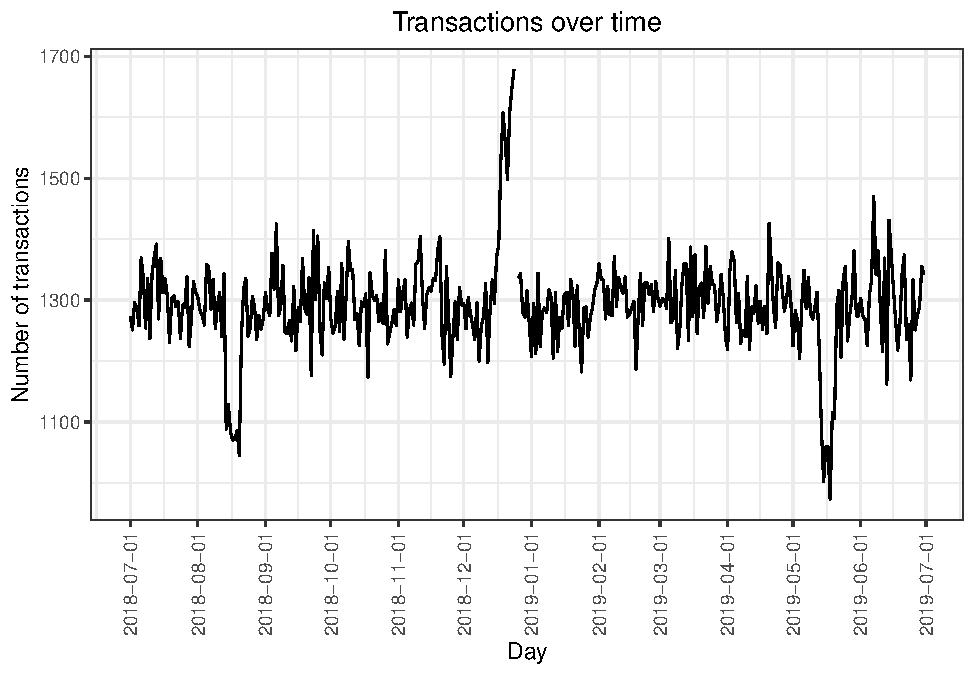
\includegraphics{template_files/figure-latex/unnamed-chunk-7-1} \end{center}

We can see that there is an increase in purchases in December and a
break in late December. Let's zoom in on this.

\begin{Shaded}
\begin{Highlighting}[]
\DocumentationTok{\#\#\#\# Filter to December and look at individual days}
\CommentTok{\# Over to you {-} recreate the chart above zoomed in to the relevant dates.}

\FunctionTok{ggplot}\NormalTok{(transactions\_by\_day, }\FunctionTok{aes}\NormalTok{(}\AttributeTok{x =}\NormalTok{ DATE, }\AttributeTok{y =}\NormalTok{ COUNT)) }\SpecialCharTok{+}
 \FunctionTok{geom\_line}\NormalTok{() }\SpecialCharTok{+}
 \FunctionTok{labs}\NormalTok{(}\AttributeTok{x =} \StringTok{"Day"}\NormalTok{, }\AttributeTok{y =} \StringTok{"Number of transactions"}\NormalTok{, }\AttributeTok{title =} \StringTok{"Transactions over time"}\NormalTok{) }\SpecialCharTok{+}
 \FunctionTok{scale\_x\_date}\NormalTok{(}\AttributeTok{breaks =} \StringTok{"1 day"}\NormalTok{, }\AttributeTok{limits =} \FunctionTok{as.Date}\NormalTok{(}\FunctionTok{c}\NormalTok{(}\StringTok{"2018{-}12{-}01"}\NormalTok{,}\StringTok{"2018{-}12{-}31"}\NormalTok{))) }\SpecialCharTok{+}
 \FunctionTok{theme}\NormalTok{(}\AttributeTok{axis.text.x =} \FunctionTok{element\_text}\NormalTok{(}\AttributeTok{angle =} \DecValTok{90}\NormalTok{, }\AttributeTok{vjust =} \FloatTok{0.5}\NormalTok{))}
\end{Highlighting}
\end{Shaded}

\begin{verbatim}
## Warning: Removed 334 rows containing missing values (`geom_line()`).
\end{verbatim}

\begin{center}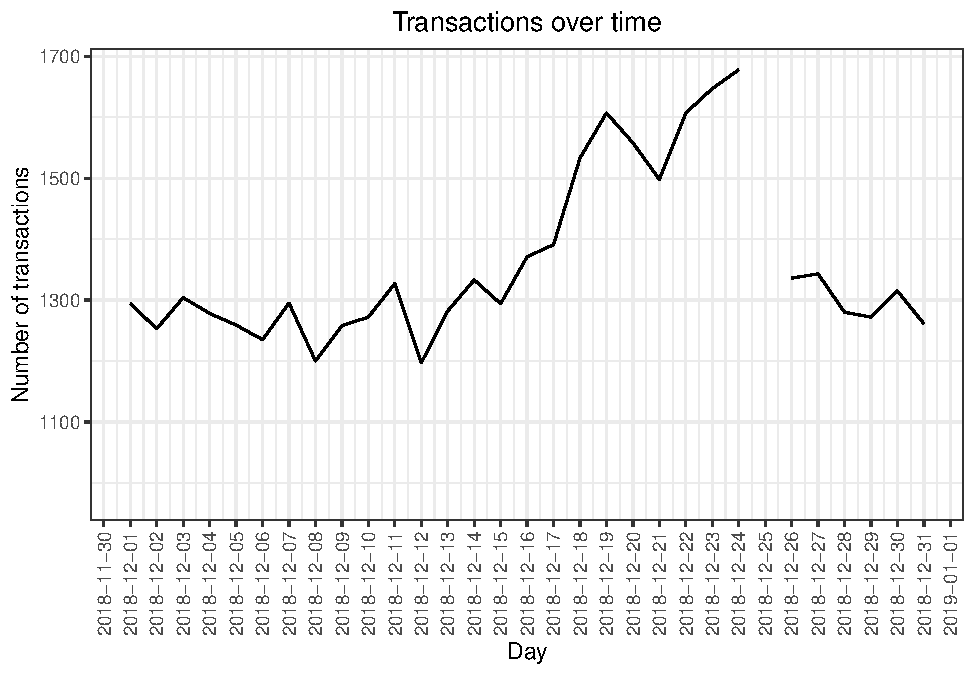
\includegraphics{template_files/figure-latex/unnamed-chunk-8-1} \end{center}

We can see that the increase in sales occurs in the lead-up to Christmas
and that there are zero sales on Christmas day itself. This is due to
shops being closed on Christmas day. Now that we are satisfied that the
data no longer has outliers, we can move on to creating other features
such as brand of chips or pack size from PROD\_NAME. We will start with
pack size.

\begin{Shaded}
\begin{Highlighting}[]
\DocumentationTok{\#\#\#\# Pack size}
\DocumentationTok{\#\#\#\# We can work this out by taking the digits that are in PROD\_NAME}
\NormalTok{transactionData[, PACK\_SIZE }\SpecialCharTok{:=} \FunctionTok{parse\_number}\NormalTok{(PROD\_NAME)]}
\DocumentationTok{\#\#\#\# Always check your output}
\DocumentationTok{\#\#\#\# Let\textquotesingle{}s check if the pack sizes look sensible}
\NormalTok{transactionData[, .N, PACK\_SIZE][}\FunctionTok{order}\NormalTok{(PACK\_SIZE)]}
\end{Highlighting}
\end{Shaded}

\begin{verbatim}
##     PACK_SIZE     N
##  1:        70  1507
##  2:        90  3008
##  3:       110 22387
##  4:       125  1454
##  5:       134 25102
##  6:       135  3257
##  7:       150 40203
##  8:       160  2970
##  9:       165 15297
## 10:       170 19983
## 11:       175 66390
## 12:       180  1468
## 13:       190  2995
## 14:       200  4473
## 15:       210  6272
## 16:       220  1564
## 17:       250  3169
## 18:       270  6285
## 19:       330 12540
## 20:       380  6416
\end{verbatim}

The largest size is 380g and the smallest size is 70g - seems sensible!

\begin{Shaded}
\begin{Highlighting}[]
\DocumentationTok{\#\#\#\# Let\textquotesingle{}s plot a histogram of PACK\_SIZE since we know that it is a categorical variable and not a continuous variable even though it is numeric.}
\CommentTok{\# Over to you! Plot a histogram showing the number of transactions by pack size.}

\FunctionTok{ggplot}\NormalTok{(transactionData[, .N, PACK\_SIZE]) }\SpecialCharTok{+} \FunctionTok{geom\_histogram}\NormalTok{(}\FunctionTok{aes}\NormalTok{(}\AttributeTok{x =}\NormalTok{ PACK\_SIZE, }\AttributeTok{y =}\NormalTok{ N), }\AttributeTok{stat=}\StringTok{"identity"}\NormalTok{) }\SpecialCharTok{+} \FunctionTok{labs}\NormalTok{(}\AttributeTok{x =} \StringTok{"Pack Size"}\NormalTok{, }\AttributeTok{y =} \StringTok{"Count"}\NormalTok{, }\AttributeTok{title =} \StringTok{"Pack Size Count"}\NormalTok{)}
\end{Highlighting}
\end{Shaded}

\begin{verbatim}
## Warning in geom_histogram(aes(x = PACK_SIZE, y = N), stat = "identity"):
## Ignoring unknown parameters: `binwidth`, `bins`, and `pad`
\end{verbatim}

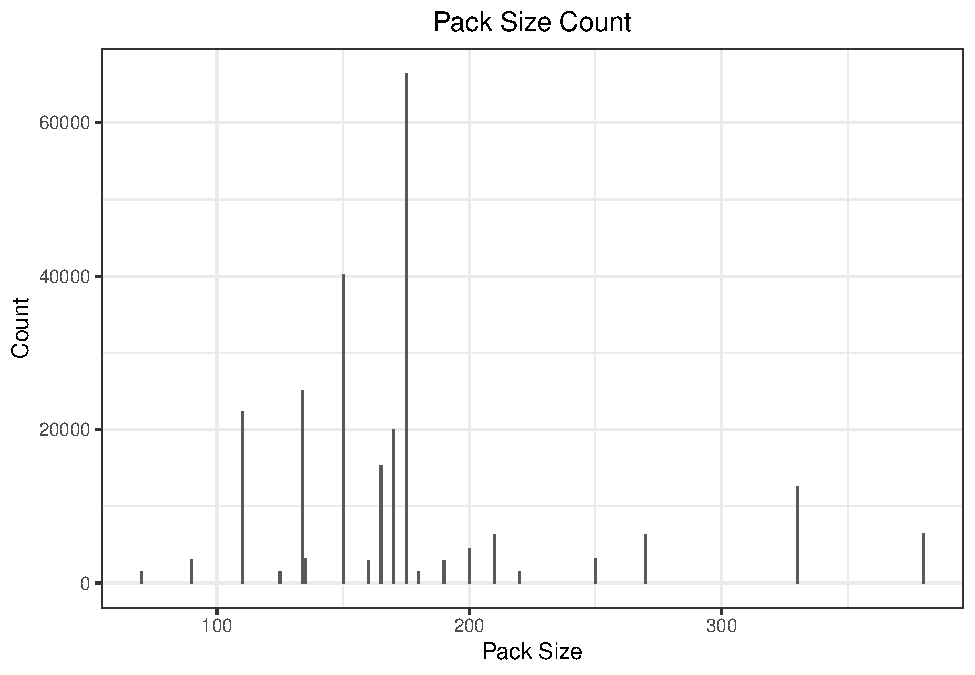
\includegraphics{template_files/figure-latex/unnamed-chunk-9-1.pdf} Pack
sizes created look reasonable. Now to create brands, we can use the
first word in PROD\_NAME to work out the brand name\ldots{}

\begin{Shaded}
\begin{Highlighting}[]
\DocumentationTok{\#\#\#\# Brands}
\CommentTok{\# Over to you! Create a column which contains the brand of the product, by extracting it from the product name.}

\CommentTok{\# subset the first word from the name as the brand}
\CommentTok{\# parse through names of each row and strsplit}
\NormalTok{transactionData }\OtherTok{\textless{}{-}}\NormalTok{ transactionData }\SpecialCharTok{\%\textgreater{}\%} \FunctionTok{mutate}\NormalTok{(}\AttributeTok{BRAND =} \FunctionTok{str\_split}\NormalTok{(PROD\_NAME, }\StringTok{" "}\NormalTok{, }\AttributeTok{simplify =} \ConstantTok{TRUE}\NormalTok{)[,}\DecValTok{1}\NormalTok{])}

\DocumentationTok{\#\#\#\# Checking brands}
\CommentTok{\# Over to you! Check the results look reasonable.}

\FunctionTok{unique}\NormalTok{(transactionData[,BRAND])}
\end{Highlighting}
\end{Shaded}

\begin{verbatim}
##  [1] "Natural"    "CCs"        "Smiths"     "Kettle"     "Grain"     
##  [6] "Doritos"    "Twisties"   "WW"         "Thins"      "Burger"    
## [11] "NCC"        "Cheezels"   "Infzns"     "Red"        "Pringles"  
## [16] "Dorito"     "Infuzions"  "Smith"      "GrnWves"    "Tyrrells"  
## [21] "Cobs"       "French"     "RRD"        "Tostitos"   "Cheetos"   
## [26] "Woolworths" "Snbts"      "Sunbites"
\end{verbatim}

Some of the brand names look like they are of the same brands - such as
RED and RRD, which are both Red Rock Deli chips. Let's combine these
together.

\begin{Shaded}
\begin{Highlighting}[]
\DocumentationTok{\#\#\#\# Clean brand names}
\NormalTok{transactionData[BRAND }\SpecialCharTok{==} \StringTok{"RED"}\NormalTok{, BRAND }\SpecialCharTok{:=} \StringTok{"RRD"}\NormalTok{]}
\CommentTok{\# Over to you! Add any additional brand adjustments you think may be required.}

\NormalTok{transactionData[BRAND }\SpecialCharTok{==} \StringTok{"Infuzions"}\NormalTok{, BRAND }\SpecialCharTok{:=} \StringTok{"Infzns"}\NormalTok{]}

\NormalTok{transactionData[BRAND }\SpecialCharTok{==} \StringTok{"Woolworths"}\NormalTok{, BRAND }\SpecialCharTok{:=} \StringTok{"WW"}\NormalTok{]}

\NormalTok{transactionData[BRAND }\SpecialCharTok{==} \StringTok{"Natural"}\NormalTok{, BRAND }\SpecialCharTok{:=} \StringTok{"NCC"}\NormalTok{]}

\NormalTok{transactionData[BRAND }\SpecialCharTok{==} \StringTok{"Grain"}\NormalTok{, BRAND }\SpecialCharTok{:=} \StringTok{"GrnWves"}\NormalTok{]}

\NormalTok{transactionData[BRAND }\SpecialCharTok{==} \StringTok{"Sunbites"}\NormalTok{, BRAND }\SpecialCharTok{:=} \StringTok{"Snbts"}\NormalTok{]}

\NormalTok{transactionData[BRAND }\SpecialCharTok{==} \StringTok{"Smith"}\NormalTok{, BRAND}\SpecialCharTok{:=}\StringTok{"Smiths"}\NormalTok{]}

\DocumentationTok{\#\#\#\# Check again}
\CommentTok{\# Over to you! Check the results look reasonable.}

\FunctionTok{unique}\NormalTok{(transactionData[,}\StringTok{"BRAND"}\NormalTok{])}
\end{Highlighting}
\end{Shaded}

\begin{verbatim}
##        BRAND
##  1:      NCC
##  2:      CCs
##  3:   Smiths
##  4:   Kettle
##  5:  GrnWves
##  6:  Doritos
##  7: Twisties
##  8:       WW
##  9:    Thins
## 10:   Burger
## 11: Cheezels
## 12:   Infzns
## 13:      Red
## 14: Pringles
## 15:   Dorito
## 16: Tyrrells
## 17:     Cobs
## 18:   French
## 19:      RRD
## 20: Tostitos
## 21:  Cheetos
## 22:    Snbts
##        BRAND
\end{verbatim}

\hypertarget{examining-customer-data}{%
\subsubsection{Examining customer data}\label{examining-customer-data}}

Now that we are happy with the transaction dataset, let's have a look at
the customer dataset.

\begin{Shaded}
\begin{Highlighting}[]
\DocumentationTok{\#\#\#\# Examining customer data}
\CommentTok{\# Over to you! Do some basic summaries of the dataset, including distributions of any key columns.}

\FunctionTok{summary}\NormalTok{(transactionData)}
\end{Highlighting}
\end{Shaded}

\begin{verbatim}
##       DATE              STORE_NBR     LYLTY_CARD_NBR        TXN_ID       
##  Min.   :2018-07-01   Min.   :  1.0   Min.   :   1000   Min.   :      1  
##  1st Qu.:2018-09-30   1st Qu.: 70.0   1st Qu.:  70015   1st Qu.:  67569  
##  Median :2018-12-30   Median :130.0   Median : 130367   Median : 135182  
##  Mean   :2018-12-30   Mean   :135.1   Mean   : 135530   Mean   : 135130  
##  3rd Qu.:2019-03-31   3rd Qu.:203.0   3rd Qu.: 203083   3rd Qu.: 202652  
##  Max.   :2019-06-30   Max.   :272.0   Max.   :2373711   Max.   :2415841  
##     PROD_NBR       PROD_NAME            PROD_QTY       TOT_SALES     
##  Min.   :  1.00   Length:246740      Min.   :1.000   Min.   : 1.700  
##  1st Qu.: 26.00   Class :character   1st Qu.:2.000   1st Qu.: 5.800  
##  Median : 53.00   Mode  :character   Median :2.000   Median : 7.400  
##  Mean   : 56.35                      Mean   :1.906   Mean   : 7.316  
##  3rd Qu.: 87.00                      3rd Qu.:2.000   3rd Qu.: 8.800  
##  Max.   :114.00                      Max.   :5.000   Max.   :29.500  
##    PACK_SIZE        BRAND          
##  Min.   : 70.0   Length:246740     
##  1st Qu.:150.0   Class :character  
##  Median :170.0   Mode  :character  
##  Mean   :175.6                     
##  3rd Qu.:175.0                     
##  Max.   :380.0
\end{verbatim}

\begin{Shaded}
\begin{Highlighting}[]
\CommentTok{\# get distribution for total purchase for each store}
\NormalTok{store\_nbr\_dist }\OtherTok{\textless{}{-}} \FunctionTok{table}\NormalTok{(transactionData}\SpecialCharTok{$}\NormalTok{STORE\_NBR)}
\CommentTok{\# graph}
\FunctionTok{ggplot}\NormalTok{() }\SpecialCharTok{+} \FunctionTok{geom\_bar}\NormalTok{(}\FunctionTok{aes}\NormalTok{(}\AttributeTok{x =} \FunctionTok{as.numeric}\NormalTok{(}\FunctionTok{names}\NormalTok{(store\_nbr\_dist)), }\AttributeTok{y =}\NormalTok{ store\_nbr\_dist), }\AttributeTok{stat =} \StringTok{"identity"}\NormalTok{) }\SpecialCharTok{+} \FunctionTok{labs}\NormalTok{(}\AttributeTok{x =} \StringTok{"Store Number"}\NormalTok{, }\AttributeTok{y =} \StringTok{"Total Purchases for each Store"}\NormalTok{, }\AttributeTok{title =} \StringTok{"Purchases per Store"}\NormalTok{)}
\end{Highlighting}
\end{Shaded}

\begin{verbatim}
## Don't know how to automatically pick scale for object of type <table>.
## Defaulting to continuous.
\end{verbatim}

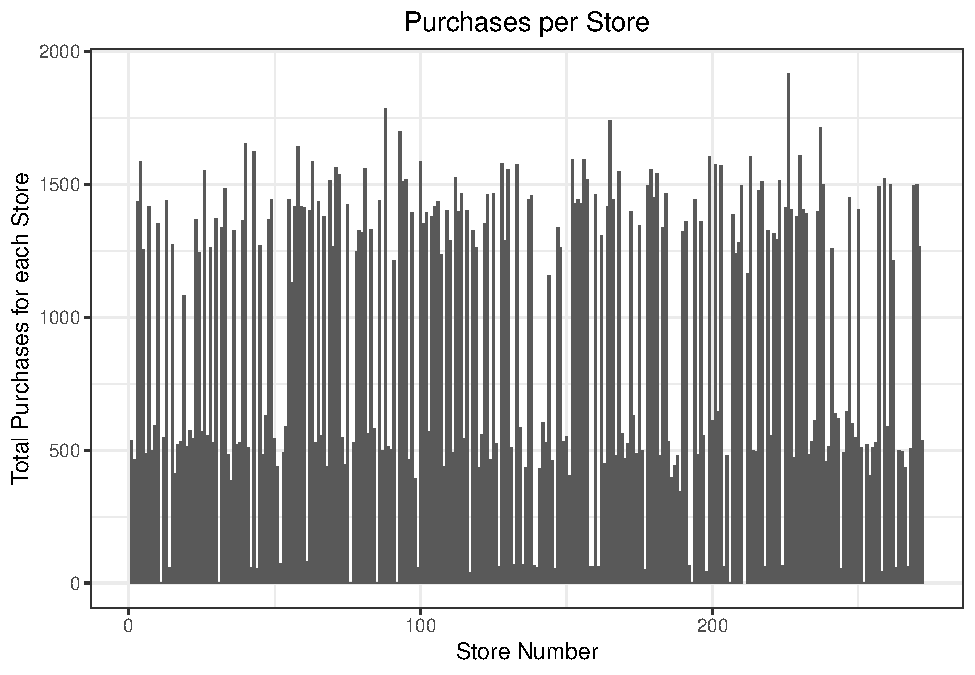
\includegraphics{template_files/figure-latex/1 Exploratory data analysis-1.pdf}

\begin{Shaded}
\begin{Highlighting}[]
\CommentTok{\# store number 271 is missing}
\end{Highlighting}
\end{Shaded}

\begin{Shaded}
\begin{Highlighting}[]
\DocumentationTok{\#\#\#\# Merge transaction data to customer data}
\NormalTok{data }\OtherTok{\textless{}{-}} \FunctionTok{merge}\NormalTok{(transactionData, customerData, }\AttributeTok{all.x =} \ConstantTok{TRUE}\NormalTok{)}
\end{Highlighting}
\end{Shaded}

As the number of rows in \texttt{data} is the same as that of
\texttt{transactionData}, we can be sure that no duplicates were
created. This is because we created \texttt{data} by setting
\texttt{all.x\ =\ TRUE} (in other words, a left join) which means take
all the rows in \texttt{transactionData} and find rows with matching
values in shared columns and then joining the details in these rows to
the \texttt{x} or the first mentioned table.

Let's also check if some customers were not matched on by checking for
nulls.

\begin{Shaded}
\begin{Highlighting}[]
\CommentTok{\# Over to you! See if any transactions did not have a matched customer.}

\ControlFlowTok{for}\NormalTok{(col }\ControlFlowTok{in} \FunctionTok{colnames}\NormalTok{(transactionData))}
\NormalTok{\{}
  \FunctionTok{print}\NormalTok{(}\FunctionTok{any}\NormalTok{(}\FunctionTok{is.na}\NormalTok{(data[,..col])))}
  \FunctionTok{print}\NormalTok{(}\FunctionTok{any}\NormalTok{(}\FunctionTok{is.null}\NormalTok{(data[,..col])))}
\NormalTok{\}}
\end{Highlighting}
\end{Shaded}

\begin{verbatim}
## [1] FALSE
## [1] FALSE
## [1] FALSE
## [1] FALSE
## [1] FALSE
## [1] FALSE
## [1] FALSE
## [1] FALSE
## [1] FALSE
## [1] FALSE
## [1] FALSE
## [1] FALSE
## [1] FALSE
## [1] FALSE
## [1] FALSE
## [1] FALSE
## [1] FALSE
## [1] FALSE
## [1] FALSE
## [1] FALSE
\end{verbatim}

Great, there are no nulls! So all our customers in the transaction data
has been accounted for in the customer dataset. Note that if you are
continuing with Task 2, you may want to retain this dataset which you
can write out as a csv

\begin{Shaded}
\begin{Highlighting}[]
\FunctionTok{fwrite}\NormalTok{(data, }\FunctionTok{paste0}\NormalTok{(filePath,}\StringTok{"QVI\_data.csv"}\NormalTok{))}
\end{Highlighting}
\end{Shaded}

Data exploration is now complete!

\hypertarget{data-analysis-on-customer-segments}{%
\subsection{Data analysis on customer
segments}\label{data-analysis-on-customer-segments}}

Now that the data is ready for analysis, we can define some metrics of
interest to the client: - Who spends the most on chips (total sales),
describing customers by lifestage and how premium their general
purchasing behaviour is - How many customers are in each segment - How
many chips are bought per customer by segment - What's the average chip
price by customer segment We could also ask our data team for more
information. Examples are: - The customer's total spend over the period
and total spend for each transaction to understand what proportion of
their grocery spend is on chips - Proportion of customers in each
customer segment overall to compare against the mix of customers who
purchase chips Let's start with calculating total sales by LIFESTAGE and
PREMIUM\_CUSTOMER and plotting the split by these segments to describe
which customer segment contribute most to chip sales.

\begin{Shaded}
\begin{Highlighting}[]
\DocumentationTok{\#\#\#\# Total sales by LIFESTAGE and PREMIUM\_CUSTOMER}
\CommentTok{\# Over to you! Calculate the summary of sales by those dimensions and create a plot.}

\NormalTok{cust\_seg }\OtherTok{\textless{}{-}}\NormalTok{ data[,}\FunctionTok{c}\NormalTok{(}\StringTok{"TOT\_SALES"}\NormalTok{,}\StringTok{"LIFESTAGE"}\NormalTok{,}\StringTok{"PREMIUM\_CUSTOMER"}\NormalTok{)]}

\CommentTok{\# parse through info, for each premium type and lifestyle}
\NormalTok{sumPremLife }\OtherTok{\textless{}{-}} \ControlFlowTok{function}\NormalTok{(df)}
\NormalTok{\{}
  
  \CommentTok{\# make data frame holding:}
  \CommentTok{\# total sales, customer segment}
\NormalTok{  res }\OtherTok{\textless{}{-}} \FunctionTok{data.frame}\NormalTok{(}\FunctionTok{matrix}\NormalTok{(}\AttributeTok{ncol =} \DecValTok{3}\NormalTok{))}
  
  \ControlFlowTok{for}\NormalTok{(premStat }\ControlFlowTok{in} \FunctionTok{unique}\NormalTok{(df}\SpecialCharTok{$}\NormalTok{PREMIUM\_CUSTOMER))}
\NormalTok{  \{}
    \ControlFlowTok{for}\NormalTok{(lifeStat }\ControlFlowTok{in} \FunctionTok{unique}\NormalTok{(df}\SpecialCharTok{$}\NormalTok{LIFESTAGE))}
\NormalTok{    \{}
      \CommentTok{\# filter data by premstat and lifestat}
\NormalTok{      m }\OtherTok{\textless{}{-}}\NormalTok{ df }\SpecialCharTok{\%\textgreater{}\%} \FunctionTok{filter}\NormalTok{(PREMIUM\_CUSTOMER }\SpecialCharTok{==}\NormalTok{ premStat }\SpecialCharTok{\&}\NormalTok{ LIFESTAGE }\SpecialCharTok{==}\NormalTok{ lifeStat)}
      
      \CommentTok{\# sum total sales}
\NormalTok{      totSales }\OtherTok{\textless{}{-}} \FunctionTok{sum}\NormalTok{(m}\SpecialCharTok{$}\NormalTok{TOT\_SALES)}
      
      \CommentTok{\# add onto matrix }
\NormalTok{      res }\OtherTok{\textless{}{-}} \FunctionTok{rbind}\NormalTok{(res,}\FunctionTok{c}\NormalTok{(}\FunctionTok{paste0}\NormalTok{(premStat, }\StringTok{" {-} "}\NormalTok{, lifeStat), totSales, }\FunctionTok{nrow}\NormalTok{(m)))}
      
\NormalTok{    \}}
\NormalTok{  \}}
  
  \CommentTok{\# remove first row}
\NormalTok{  res }\OtherTok{\textless{}{-}}\NormalTok{ res[}\DecValTok{2}\SpecialCharTok{:}\FunctionTok{nrow}\NormalTok{(res),]}
  \CommentTok{\# reset indices}
  \FunctionTok{rownames}\NormalTok{(res) }\OtherTok{\textless{}{-}} \ConstantTok{NULL}
  \CommentTok{\# name columns}
  \FunctionTok{colnames}\NormalTok{(res) }\OtherTok{\textless{}{-}} \FunctionTok{c}\NormalTok{(}\StringTok{"Customer\_Segment"}\NormalTok{,}\StringTok{"Total\_Sales"}\NormalTok{, }\StringTok{"N\_Customer"}\NormalTok{)}
  
  \FunctionTok{return}\NormalTok{(res)}
\NormalTok{\}}

\NormalTok{segdata }\OtherTok{\textless{}{-}} \FunctionTok{sumPremLife}\NormalTok{(cust\_seg)}


\CommentTok{\# plot}
\FunctionTok{ggplot}\NormalTok{(segdata) }\SpecialCharTok{+} \FunctionTok{geom\_bar}\NormalTok{(}\FunctionTok{aes}\NormalTok{(}\AttributeTok{x =}\NormalTok{ Customer\_Segment, }\AttributeTok{y =}\NormalTok{ Total\_Sales), }\AttributeTok{stat =} \StringTok{"identity"}\NormalTok{) }\SpecialCharTok{+} \FunctionTok{theme}\NormalTok{(}\AttributeTok{axis.text.x =} \FunctionTok{element\_text}\NormalTok{(}\AttributeTok{angle =} \DecValTok{90}\NormalTok{)) }\SpecialCharTok{+} \FunctionTok{labs}\NormalTok{(}\AttributeTok{title =} \StringTok{"Total Sales per Customer Premium/Lifestage Type"}\NormalTok{, }\AttributeTok{x =} \StringTok{"Premium/Lifestage Type"}\NormalTok{, }\AttributeTok{y =} \StringTok{"Total Sales"}\NormalTok{)}
\end{Highlighting}
\end{Shaded}

\begin{center}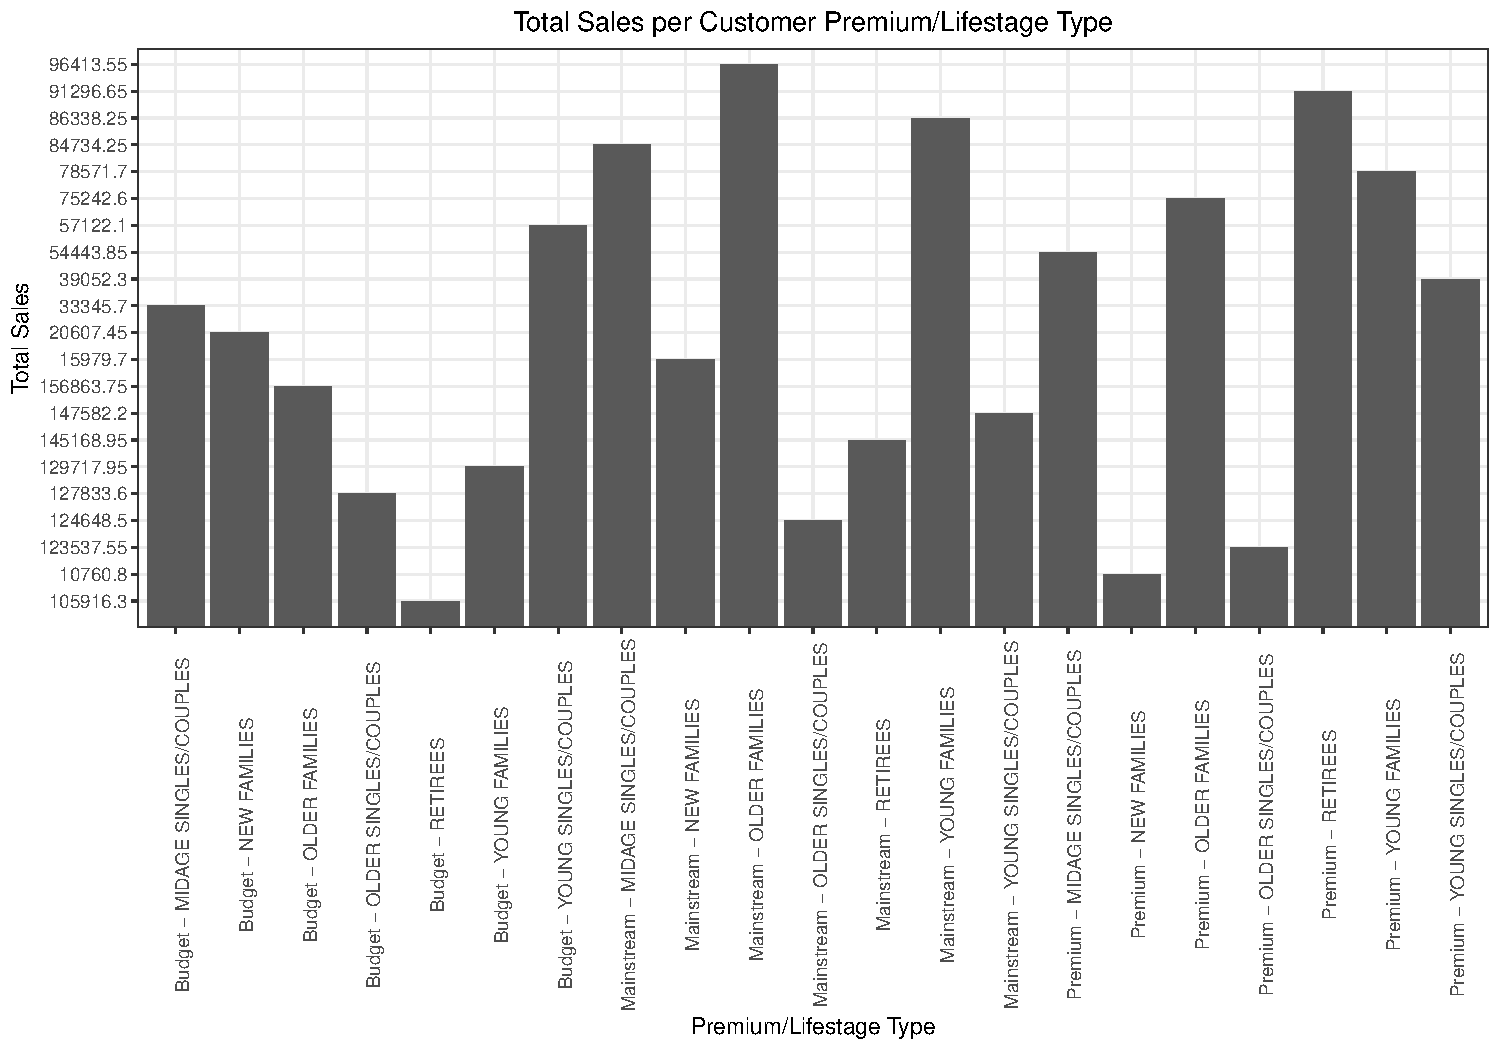
\includegraphics{template_files/figure-latex/unnamed-chunk-11-1} \end{center}

Sales are coming mainly from Budget - older families, Mainstream - young
singles/couples, and Mainstream - Older retirees. Let's see if the
higher sales are due to there being more customers who buy chips.

\begin{Shaded}
\begin{Highlighting}[]
\DocumentationTok{\#\#\#\# Number of customers by LIFESTAGE and PREMIUM\_CUSTOMER}
\CommentTok{\# Over to you! Calculate the summary of number of customers by those dimensions and create a plot.}

\CommentTok{\# subset all products with "chip" in product name}
\NormalTok{cust\_seg\_chip }\OtherTok{\textless{}{-}}\NormalTok{ data[}\FunctionTok{grepl}\NormalTok{(}\StringTok{"CHIP"}\NormalTok{,}\FunctionTok{toupper}\NormalTok{(data}\SpecialCharTok{$}\NormalTok{PROD\_NAME)),}\FunctionTok{c}\NormalTok{(}\StringTok{"TOT\_SALES"}\NormalTok{,}\StringTok{"LIFESTAGE"}\NormalTok{,}\StringTok{"PREMIUM\_CUSTOMER"}\NormalTok{)]}

\CommentTok{\# prem life sum sales based on chip}
\NormalTok{chip\_premlife }\OtherTok{\textless{}{-}} \FunctionTok{sumPremLife}\NormalTok{(cust\_seg\_chip)}

\CommentTok{\# plot}
\FunctionTok{ggplot}\NormalTok{(chip\_premlife) }\SpecialCharTok{+} \FunctionTok{geom\_bar}\NormalTok{(}\FunctionTok{aes}\NormalTok{(}\AttributeTok{x =}\NormalTok{ Customer\_Segment, }\AttributeTok{y =}\NormalTok{ Total\_Sales), }\AttributeTok{stat =} \StringTok{"identity"}\NormalTok{) }\SpecialCharTok{+} \FunctionTok{theme}\NormalTok{(}\AttributeTok{axis.text.x =} \FunctionTok{element\_text}\NormalTok{(}\AttributeTok{angle =} \DecValTok{90}\NormalTok{)) }\SpecialCharTok{+} \FunctionTok{labs}\NormalTok{(}\AttributeTok{title =} \StringTok{"Total Sales per Customer Premium/Lifestage Type of Chips"}\NormalTok{, }\AttributeTok{x =} \StringTok{"Premium/Lifestage Type"}\NormalTok{, }\AttributeTok{y =} \StringTok{"Total Sales"}\NormalTok{)}
\end{Highlighting}
\end{Shaded}

\begin{center}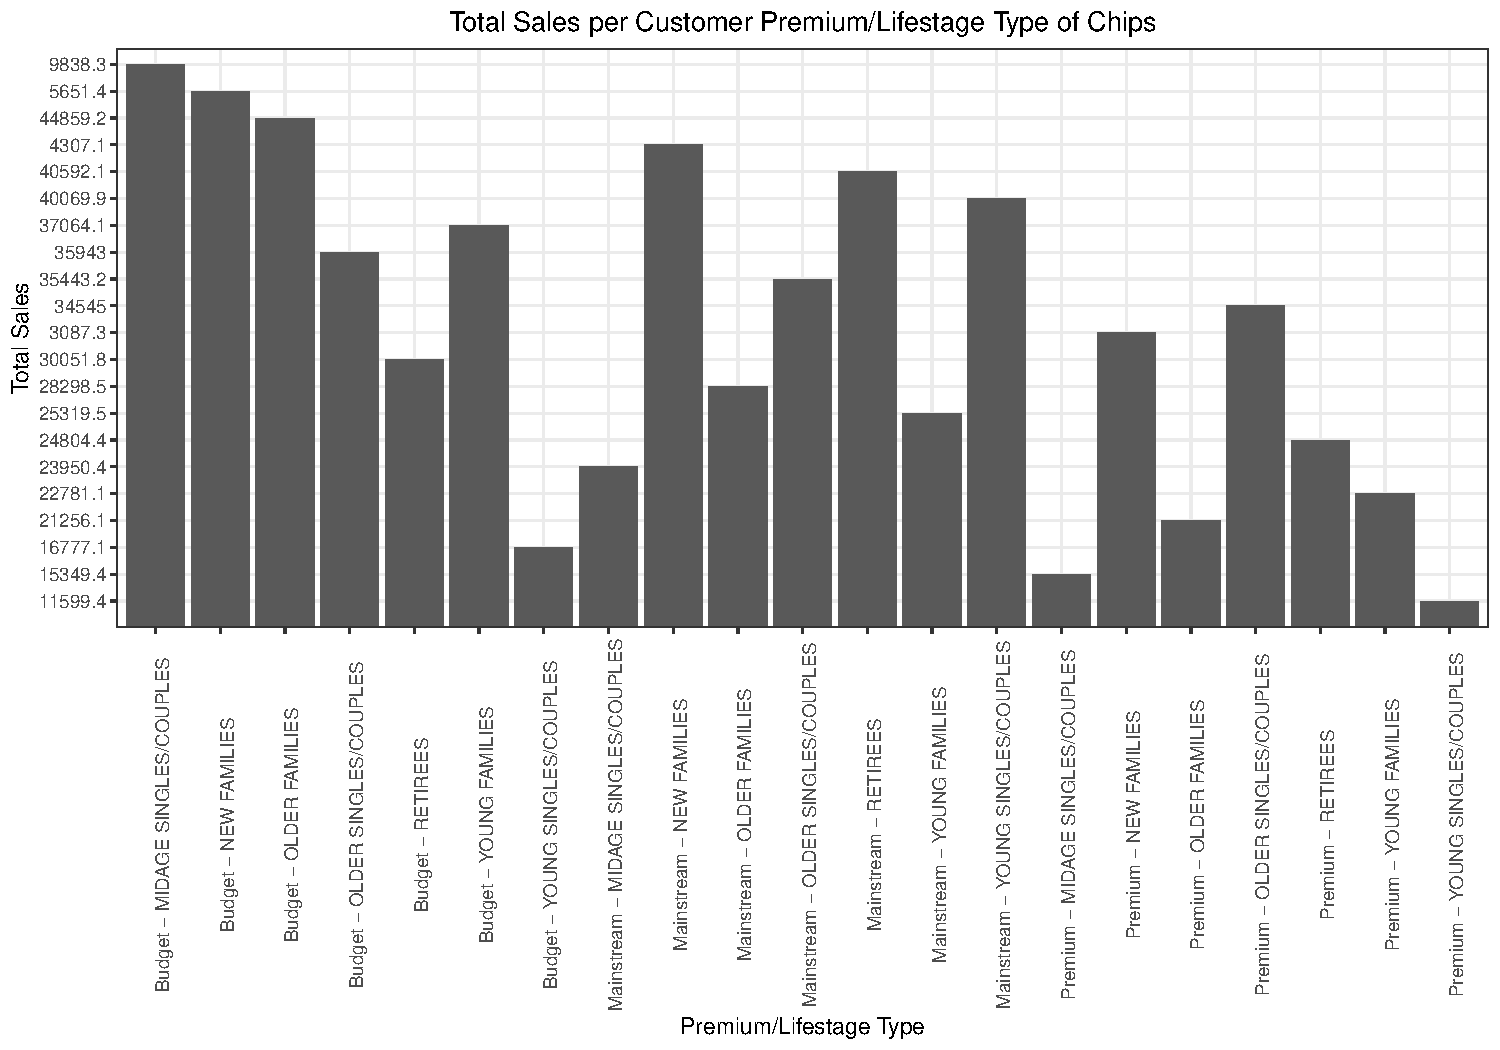
\includegraphics{template_files/figure-latex/unnamed-chunk-12-1} \end{center}

There are more Budget - Older families, Mainstream - young
singles/couples and Mainstream - retirees who buy chips. This
contributes to there being more sales to these customer segments but
this is not a major driver for the Budget - Older families segment.
Higher sales may also be driven by more units of chips being bought per
customer. Let's have a look at this next.

\begin{Shaded}
\begin{Highlighting}[]
\DocumentationTok{\#\#\#\# Average number of units per customer by LIFESTAGE and PREMIUM\_CUSTOMER}
\CommentTok{\# Over to you! Calculate and plot the average number of units per customer by those two dimensions.}

\CommentTok{\# change into numeric}
\NormalTok{segdata}\SpecialCharTok{$}\NormalTok{Total\_Sales }\OtherTok{\textless{}{-}} \FunctionTok{as.numeric}\NormalTok{(segdata}\SpecialCharTok{$}\NormalTok{Total\_Sales)}
\NormalTok{segdata}\SpecialCharTok{$}\NormalTok{N\_Customer }\OtherTok{\textless{}{-}} \FunctionTok{as.numeric}\NormalTok{(segdata}\SpecialCharTok{$}\NormalTok{N\_Customer)}

\CommentTok{\# mutate for avg column}
\NormalTok{segdata\_v1 }\OtherTok{\textless{}{-}}\NormalTok{ segdata }\SpecialCharTok{\%\textgreater{}\%} \FunctionTok{mutate}\NormalTok{(}\AttributeTok{Avg\_Total =}\NormalTok{ Total\_Sales }\SpecialCharTok{/}\NormalTok{ N\_Customer)}

\CommentTok{\# plot}
\FunctionTok{ggplot}\NormalTok{(segdata\_v1) }\SpecialCharTok{+} \FunctionTok{geom\_bar}\NormalTok{(}\FunctionTok{aes}\NormalTok{(}\AttributeTok{x =}\NormalTok{ Customer\_Segment, }\AttributeTok{y =}\NormalTok{ Avg\_Total), }\AttributeTok{stat =} \StringTok{"identity"}\NormalTok{) }\SpecialCharTok{+} \FunctionTok{theme}\NormalTok{(}\AttributeTok{axis.text.x =} \FunctionTok{element\_text}\NormalTok{(}\AttributeTok{angle =} \DecValTok{90}\NormalTok{)) }\SpecialCharTok{+} \FunctionTok{labs}\NormalTok{(}\AttributeTok{title =} \StringTok{"Average Total Sales per Customer Premium/Lifestage Type"}\NormalTok{, }\AttributeTok{x =} \StringTok{"Premium/Lifestage Type"}\NormalTok{, }\AttributeTok{y =} \StringTok{"Average Total Sales"}\NormalTok{)}
\end{Highlighting}
\end{Shaded}

\begin{center}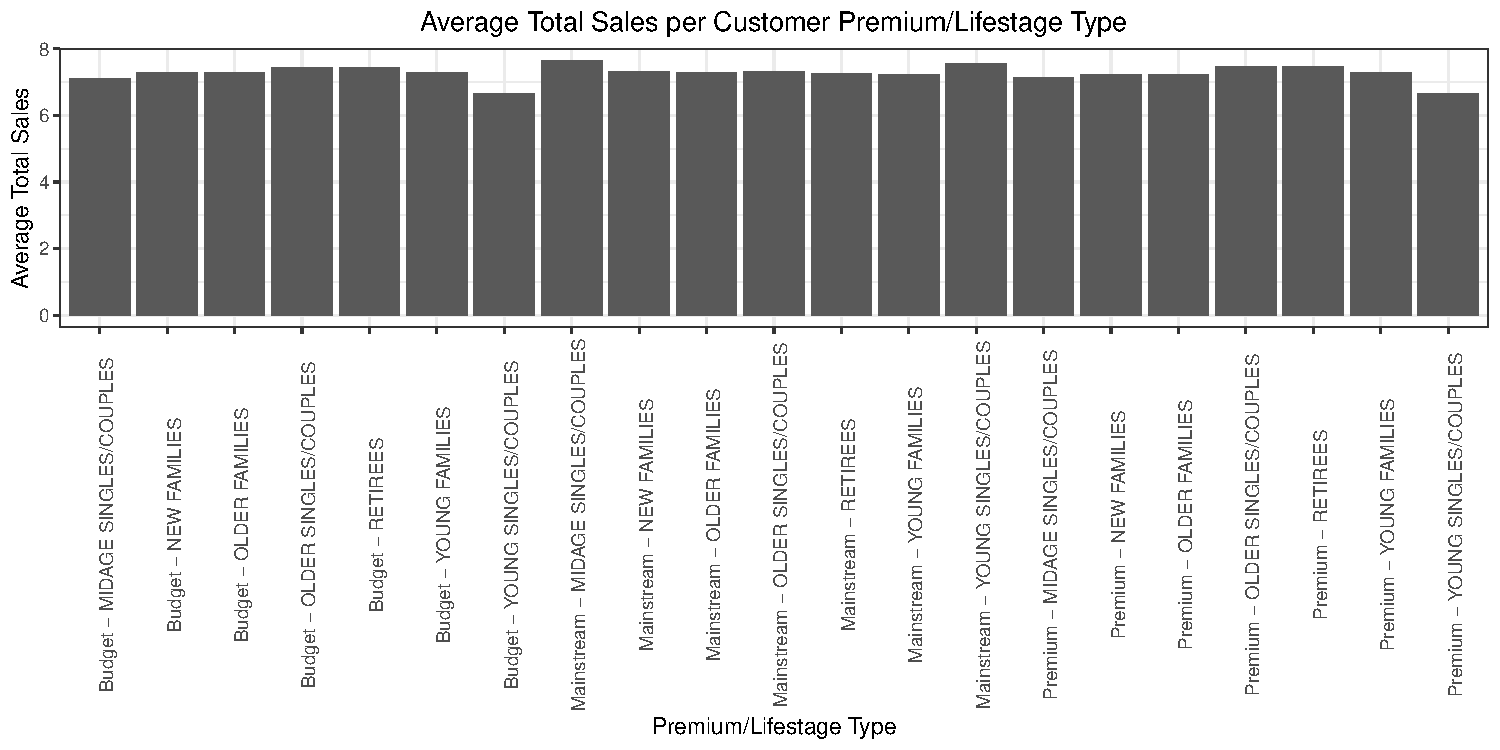
\includegraphics{template_files/figure-latex/unnamed-chunk-13-1} \end{center}

Mainstream Midage families and Young singles/couples in general buy more
chips per customer. Let's also investigate the average price per unit
chips bought for each customer segment as this is also a driver of total
sales.

\begin{Shaded}
\begin{Highlighting}[]
\DocumentationTok{\#\#\#\# Average price per unit by LIFESTAGE and PREMIUM\_CUSTOMER}
\CommentTok{\# Over to you! Calculate and plot the average price per unit sold (average sale price) by those two customer dimensions.}

\CommentTok{\# update to numeric versions}
\NormalTok{chip\_premlife }\OtherTok{\textless{}{-}}\NormalTok{ chip\_premlife }\SpecialCharTok{\%\textgreater{}\%} \FunctionTok{transform}\NormalTok{(}\AttributeTok{Total\_Sales =} \FunctionTok{as.numeric}\NormalTok{(Total\_Sales), }\AttributeTok{N\_Customer =} \FunctionTok{as.numeric}\NormalTok{(N\_Customer))}

\CommentTok{\# mutate average column}
\NormalTok{chip\_premlife\_v1 }\OtherTok{\textless{}{-}}\NormalTok{ chip\_premlife }\SpecialCharTok{\%\textgreater{}\%} \FunctionTok{mutate}\NormalTok{(}\AttributeTok{Avg\_Total =}\NormalTok{ Total\_Sales }\SpecialCharTok{/}\NormalTok{ N\_Customer)}

\CommentTok{\# plot}
\FunctionTok{ggplot}\NormalTok{(chip\_premlife\_v1) }\SpecialCharTok{+} \FunctionTok{geom\_bar}\NormalTok{(}\FunctionTok{aes}\NormalTok{(}\AttributeTok{x =}\NormalTok{ Customer\_Segment, }\AttributeTok{y =}\NormalTok{ Avg\_Total), }\AttributeTok{stat =} \StringTok{"identity"}\NormalTok{) }\SpecialCharTok{+} \FunctionTok{theme}\NormalTok{(}\AttributeTok{axis.text.x =} \FunctionTok{element\_text}\NormalTok{(}\AttributeTok{angle =} \DecValTok{90}\NormalTok{)) }\SpecialCharTok{+} \FunctionTok{labs}\NormalTok{(}\AttributeTok{title =} \StringTok{"Average Total Sales per Customer Premium/Lifestage Type {-} Chips Sales"}\NormalTok{, }\AttributeTok{x =} \StringTok{"Premium/Lifestage Type"}\NormalTok{, }\AttributeTok{y =} \StringTok{"Average Total Sales"}\NormalTok{)}
\end{Highlighting}
\end{Shaded}

\begin{center}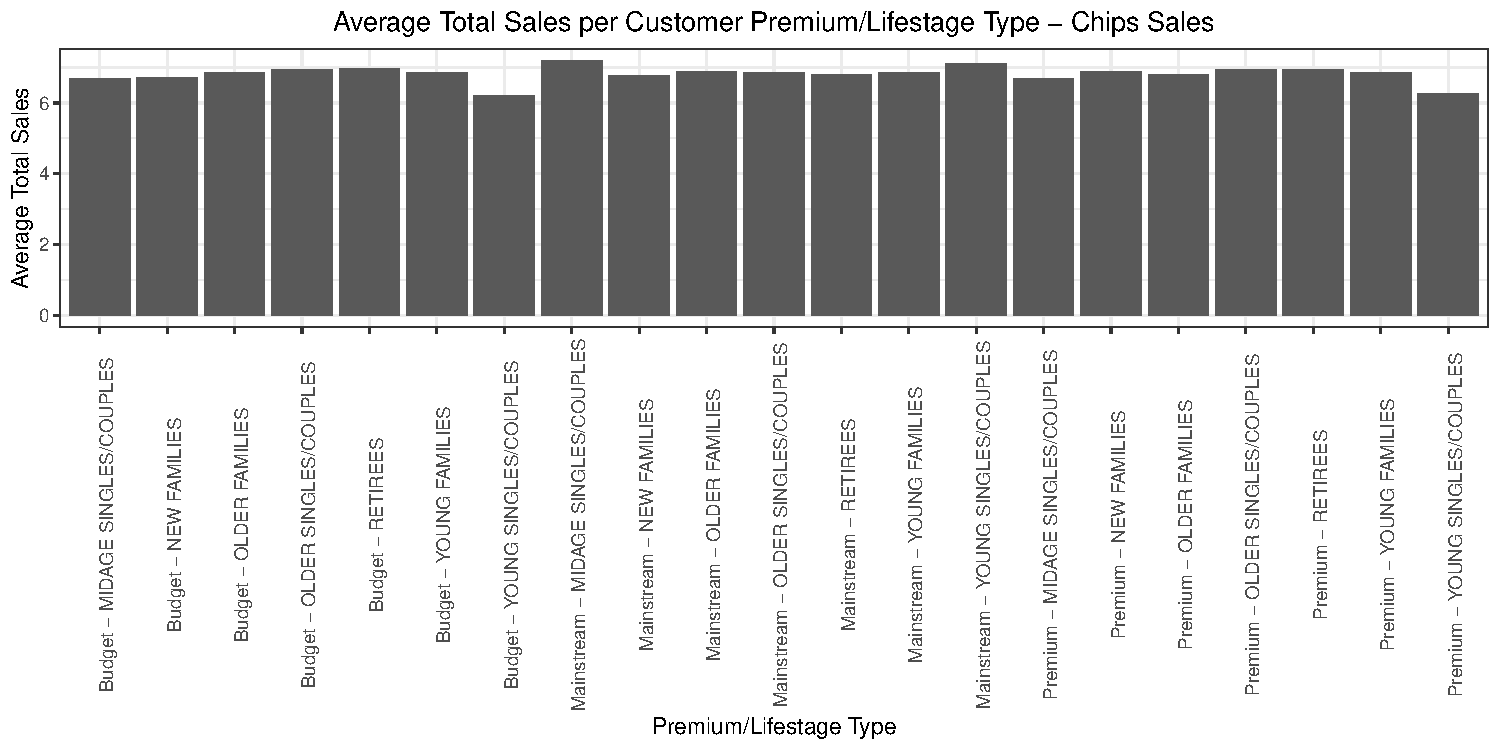
\includegraphics{template_files/figure-latex/unnamed-chunk-14-1} \end{center}

Mainstream midage and young singles and couples are more willing to pay
more per packet of chips compared to their budget and premium
counterparts. This may be due to premium shoppers being more likely to
buy healthy snacks and when they buy chips, this is mainly for
entertainment purposes rather than their own consumption. This is also
supported by there being fewer premium midage and young singles and
couples buying chips compared to their mainstream counterparts.

As the difference in average price per unit isn't large, we can check if
this difference is statistically different.

\begin{Shaded}
\begin{Highlighting}[]
\DocumentationTok{\#\#\#\# Perform an independent t{-}test between mainstream vs premium and budget midage and}
\DocumentationTok{\#\#\#\# young singles and couples}
\CommentTok{\# Over to you! Perform a t{-}test to see if the difference is significant.}

\CommentTok{\# get dataframe of chip purchases of all midage and young singles/couples}
\NormalTok{chip\_t\_test }\OtherTok{\textless{}{-}}\NormalTok{ cust\_seg\_chip[LIFESTAGE }\SpecialCharTok{==} \StringTok{"YOUNG SINGLES/COUPLES"} \SpecialCharTok{|}\NormalTok{ LIFESTAGE }\SpecialCharTok{==} \StringTok{"MIDAGE SINGLES/COUPLES"}\NormalTok{,]}

\CommentTok{\# mainstream filter}
\NormalTok{ms }\OtherTok{\textless{}{-}}\NormalTok{ chip\_t\_test[PREMIUM\_CUSTOMER }\SpecialCharTok{==} \StringTok{"Mainstream"}\NormalTok{]}

\CommentTok{\# not mainstream filter}
\NormalTok{nms }\OtherTok{\textless{}{-}}\NormalTok{ chip\_t\_test[PREMIUM\_CUSTOMER }\SpecialCharTok{!=} \StringTok{"Mainstream"}\NormalTok{]}

\CommentTok{\# test mainstream vs not mainstream}
\CommentTok{\# with equal variance}
\FunctionTok{t.test}\NormalTok{(}\AttributeTok{x =}\NormalTok{ ms}\SpecialCharTok{$}\NormalTok{TOT\_SALES, }\AttributeTok{y =}\NormalTok{ nms}\SpecialCharTok{$}\NormalTok{TOT\_SALES, }\AttributeTok{alternative =} \StringTok{"g"}\NormalTok{, }\AttributeTok{var.equal =}\NormalTok{ T, }\AttributeTok{conf.level =} \FloatTok{0.95}\NormalTok{)}
\end{Highlighting}
\end{Shaded}

\begin{verbatim}
## 
##  Two Sample t-test
## 
## data:  ms$TOT_SALES and nms$TOT_SALES
## t = 19.86, df = 17303, p-value < 2.2e-16
## alternative hypothesis: true difference in means is greater than 0
## 95 percent confidence interval:
##  0.6432478       Inf
## sample estimates:
## mean of x mean of y 
##  7.132386  6.431048
\end{verbatim}

\begin{Shaded}
\begin{Highlighting}[]
\CommentTok{\# not equal variance}
\FunctionTok{t.test}\NormalTok{(}\AttributeTok{x =}\NormalTok{ ms}\SpecialCharTok{$}\NormalTok{TOT\_SALES, }\AttributeTok{y =}\NormalTok{ nms}\SpecialCharTok{$}\NormalTok{TOT\_SALES, }\AttributeTok{alternative =} \StringTok{"g"}\NormalTok{, }\AttributeTok{var.equal =}\NormalTok{ F, }\AttributeTok{conf.level =} \FloatTok{0.95}\NormalTok{)}
\end{Highlighting}
\end{Shaded}

\begin{verbatim}
## 
##  Welch Two Sample t-test
## 
## data:  ms$TOT_SALES and nms$TOT_SALES
## t = 19.842, df = 17136, p-value < 2.2e-16
## alternative hypothesis: true difference in means is greater than 0
## 95 percent confidence interval:
##  0.6431959       Inf
## sample estimates:
## mean of x mean of y 
##  7.132386  6.431048
\end{verbatim}

The t-test results in a p-value of \textless{} 2.2e-16, i.e.~the unit
price for mainstream, young and mid-age singles and couples are
significantly higher than that of budget or premium, young and midage
singles and couples. \#\# Deep dive into specific customer segments for
insights We have found quite a few interesting insights that we can dive
deeper into. We might want to target customer segments that contribute
the most to sales to retain them or further increase sales. Let's look
at Mainstream - young singles/couples. For instance, let's find out if
they tend to buy a particular brand of chips.

\begin{Shaded}
\begin{Highlighting}[]
\DocumentationTok{\#\#\#\# Deep dive into Mainstream, young singles/couples}
\CommentTok{\# Over to you! Work out of there are brands that these two customer segments prefer more than others. You could use a technique called affinity analysis or a{-}priori analysis (or any other method if you prefer)}

\CommentTok{\# make frequency plot of different brands for young mid age singles/couples}
\NormalTok{life\_prem\_brand\_data }\OtherTok{\textless{}{-}}\NormalTok{ data[(LIFESTAGE }\SpecialCharTok{==} \StringTok{"YOUNG SINGLES/COUPLES"} \SpecialCharTok{|}\NormalTok{ LIFESTAGE }\SpecialCharTok{==} \StringTok{"MIDAGE SINGLES/COUPLES"}\NormalTok{) }\SpecialCharTok{\&} \FunctionTok{grepl}\NormalTok{(}\StringTok{"CHIP"}\NormalTok{,}\FunctionTok{toupper}\NormalTok{(data}\SpecialCharTok{$}\NormalTok{PROD\_NAME)),}\FunctionTok{c}\NormalTok{(}\StringTok{"LYLTY\_CARD\_NBR"}\NormalTok{,}\StringTok{"PROD\_NAME"}\NormalTok{,}\StringTok{"LIFESTAGE"}\NormalTok{,}\StringTok{"PREMIUM\_CUSTOMER"}\NormalTok{,}\StringTok{"BRAND"}\NormalTok{)]}

\NormalTok{freq\_brand }\OtherTok{\textless{}{-}} \FunctionTok{table}\NormalTok{(life\_prem\_brand\_data}\SpecialCharTok{$}\NormalTok{BRAND)}

\FunctionTok{ggplot}\NormalTok{() }\SpecialCharTok{+} \FunctionTok{geom\_bar}\NormalTok{(}\FunctionTok{aes}\NormalTok{(}\AttributeTok{x =} \FunctionTok{names}\NormalTok{(freq\_brand), }\AttributeTok{y =}\NormalTok{ freq\_brand), }\AttributeTok{stat=}\StringTok{"identity"}\NormalTok{) }\SpecialCharTok{+} \FunctionTok{labs}\NormalTok{(}\AttributeTok{title =} \StringTok{"Frequencies of Chip Brand Purchases for Young and Midage Singles/Couples"}\NormalTok{, }\AttributeTok{x =} \StringTok{"Brand Name"}\NormalTok{, }\AttributeTok{y =} \StringTok{"Frequency"}\NormalTok{)}
\end{Highlighting}
\end{Shaded}

\begin{verbatim}
## Don't know how to automatically pick scale for object of type <table>.
## Defaulting to continuous.
\end{verbatim}

\begin{center}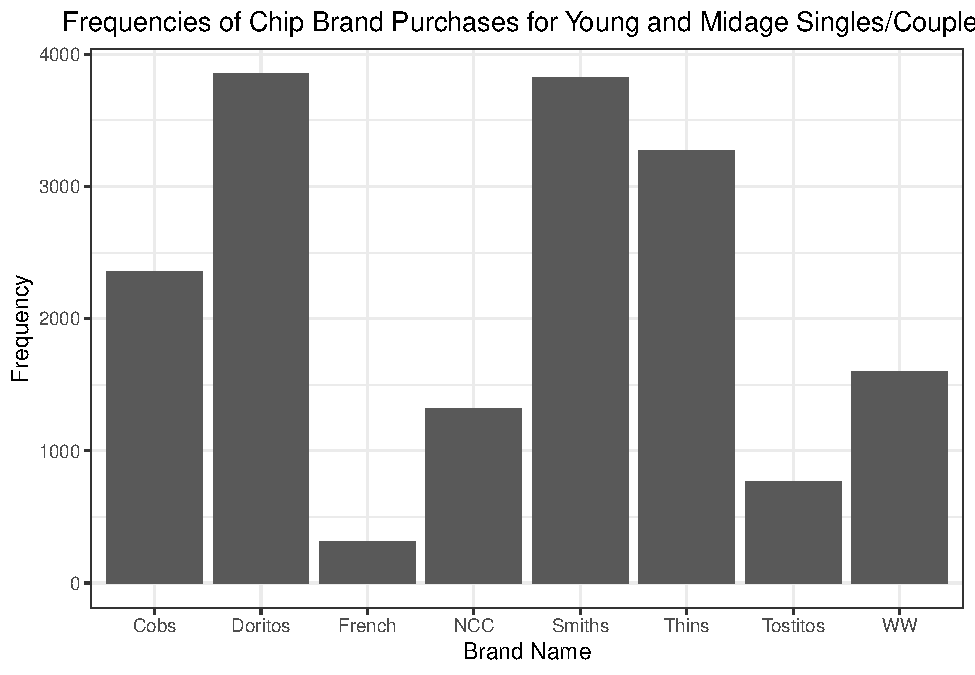
\includegraphics{template_files/figure-latex/unnamed-chunk-16-1} \end{center}

\begin{Shaded}
\begin{Highlighting}[]
\FunctionTok{sum}\NormalTok{(freq\_brand)}
\end{Highlighting}
\end{Shaded}

\begin{verbatim}
## [1] 17305
\end{verbatim}

\begin{Shaded}
\begin{Highlighting}[]
\CommentTok{\# prepare data to convert into transactions for apriori}

\CommentTok{\# get for young}

\NormalTok{young\_brand }\OtherTok{\textless{}{-}}\NormalTok{ life\_prem\_brand\_data[LIFESTAGE }\SpecialCharTok{==} \StringTok{"YOUNG SINGLES/COUPLES"}\NormalTok{,}\StringTok{"BRAND"}\NormalTok{]}
\NormalTok{young\_trans }\OtherTok{\textless{}{-}}\NormalTok{ life\_prem\_brand\_data[LIFESTAGE }\SpecialCharTok{==} \StringTok{"YOUNG SINGLES/COUPLES"}\NormalTok{,}\StringTok{"LYLTY\_CARD\_NBR"}\NormalTok{]}

\CommentTok{\# change into factors}
\NormalTok{young\_brand }\OtherTok{\textless{}{-}} \FunctionTok{factor}\NormalTok{(young\_brand}\SpecialCharTok{$}\NormalTok{BRAND)}
\NormalTok{young\_trans }\OtherTok{\textless{}{-}} \FunctionTok{factor}\NormalTok{(young\_trans}\SpecialCharTok{$}\NormalTok{LYLTY\_CARD\_NBR)}

\NormalTok{young\_transactions }\OtherTok{\textless{}{-}} \FunctionTok{split}\NormalTok{(young\_brand,young\_trans)}

\NormalTok{young\_rules }\OtherTok{\textless{}{-}} \FunctionTok{apriori}\NormalTok{(young\_transactions, }\AttributeTok{parameter =} \FunctionTok{list}\NormalTok{(}\AttributeTok{supp =} \FloatTok{0.0001}\NormalTok{, }\AttributeTok{conf =} \FloatTok{0.8}\NormalTok{))}
\end{Highlighting}
\end{Shaded}

\begin{verbatim}
## Warning in asMethod(object): removing duplicated items in transactions
\end{verbatim}

\begin{verbatim}
## Apriori
## 
## Parameter specification:
##  confidence minval smax arem  aval originalSupport maxtime support minlen
##         0.8    0.1    1 none FALSE            TRUE       5   1e-04      1
##  maxlen target  ext
##      10  rules TRUE
## 
## Algorithmic control:
##  filter tree heap memopt load sort verbose
##     0.1 TRUE TRUE  FALSE TRUE    2    TRUE
## 
## Absolute minimum support count: 0 
## 
## set item appearances ...[0 item(s)] done [0.00s].
## set transactions ...[8 item(s), 7170 transaction(s)] done [0.00s].
## sorting and recoding items ... [8 item(s)] done [0.00s].
## creating transaction tree ... done [0.00s].
## checking subsets of size 1 2 3 4 5 done [0.00s].
## writing ... [15 rule(s)] done [0.00s].
## creating S4 object  ... done [0.00s].
\end{verbatim}

\begin{Shaded}
\begin{Highlighting}[]
\CommentTok{\# remove empty col}
\NormalTok{young\_rules\_df }\OtherTok{\textless{}{-}} \FunctionTok{inspect}\NormalTok{(young\_rules) }\SpecialCharTok{\%\textgreater{}\%} \FunctionTok{select}\NormalTok{(}\SpecialCharTok{{-}}\DecValTok{2}\NormalTok{)}
\end{Highlighting}
\end{Shaded}

\begin{verbatim}
##      lhs                                 rhs       support    confidence
## [1]  {French, Smiths, Tostitos}       => {NCC}     0.00013947 1         
## [2]  {Cobs, Tostitos, WW}             => {NCC}     0.00013947 1         
## [3]  {Doritos, NCC, Tostitos}         => {WW}      0.00013947 1         
## [4]  {NCC, Thins, Tostitos}           => {Smiths}  0.00013947 1         
## [5]  {Cobs, Tostitos, WW}             => {Smiths}  0.00013947 1         
## [6]  {French, NCC, Thins, WW}         => {Smiths}  0.00027894 1         
## [7]  {French, NCC, Smiths, WW}        => {Thins}   0.00027894 1         
## [8]  {Doritos, French, NCC, Smiths}   => {Thins}   0.00013947 1         
## [9]  {Doritos, French, Smiths, Thins} => {NCC}     0.00013947 1         
## [10] {Cobs, NCC, Tostitos, WW}        => {Smiths}  0.00013947 1         
## [11] {NCC, Smiths, Tostitos, WW}      => {Cobs}    0.00013947 1         
## [12] {Cobs, NCC, Smiths, Tostitos}    => {WW}      0.00013947 1         
## [13] {Cobs, Smiths, Tostitos, WW}     => {NCC}     0.00013947 1         
## [14] {Cobs, NCC, Thins, WW}           => {Doritos} 0.00013947 1         
## [15] {Cobs, Doritos, NCC, Thins}      => {WW}      0.00013947 1         
##      coverage   lift     count
## [1]  0.00013947 9.862448 1    
## [2]  0.00013947 9.862448 1    
## [3]  0.00013947 8.405627 1    
## [4]  0.00013947 3.567164 1    
## [5]  0.00013947 3.567164 1    
## [6]  0.00027894 3.567164 2    
## [7]  0.00027894 3.952591 2    
## [8]  0.00013947 3.952591 1    
## [9]  0.00013947 9.862448 1    
## [10] 0.00013947 3.567164 1    
## [11] 0.00013947 5.395034 1    
## [12] 0.00013947 8.405627 1    
## [13] 0.00013947 9.862448 1    
## [14] 0.00013947 3.437200 1    
## [15] 0.00013947 8.405627 1
\end{verbatim}

\begin{Shaded}
\begin{Highlighting}[]
\CommentTok{\# get rules of young, focus on support for more frequent combinations}
\NormalTok{young\_rules\_df }\SpecialCharTok{\%\textgreater{}\%} \FunctionTok{arrange}\NormalTok{(}\FunctionTok{desc}\NormalTok{(support))}
\end{Highlighting}
\end{Shaded}

\begin{verbatim}
##                                   lhs       rhs    support confidence
## [6]          {French, NCC, Thins, WW}  {Smiths} 0.00027894          1
## [7]         {French, NCC, Smiths, WW}   {Thins} 0.00027894          1
## [1]        {French, Smiths, Tostitos}     {NCC} 0.00013947          1
## [2]              {Cobs, Tostitos, WW}     {NCC} 0.00013947          1
## [3]          {Doritos, NCC, Tostitos}      {WW} 0.00013947          1
## [4]            {NCC, Thins, Tostitos}  {Smiths} 0.00013947          1
## [5]              {Cobs, Tostitos, WW}  {Smiths} 0.00013947          1
## [8]    {Doritos, French, NCC, Smiths}   {Thins} 0.00013947          1
## [9]  {Doritos, French, Smiths, Thins}     {NCC} 0.00013947          1
## [10]        {Cobs, NCC, Tostitos, WW}  {Smiths} 0.00013947          1
## [11]      {NCC, Smiths, Tostitos, WW}    {Cobs} 0.00013947          1
## [12]    {Cobs, NCC, Smiths, Tostitos}      {WW} 0.00013947          1
## [13]     {Cobs, Smiths, Tostitos, WW}     {NCC} 0.00013947          1
## [14]           {Cobs, NCC, Thins, WW} {Doritos} 0.00013947          1
## [15]      {Cobs, Doritos, NCC, Thins}      {WW} 0.00013947          1
##        coverage     lift count
## [6]  0.00027894 3.567164     2
## [7]  0.00027894 3.952591     2
## [1]  0.00013947 9.862448     1
## [2]  0.00013947 9.862448     1
## [3]  0.00013947 8.405627     1
## [4]  0.00013947 3.567164     1
## [5]  0.00013947 3.567164     1
## [8]  0.00013947 3.952591     1
## [9]  0.00013947 9.862448     1
## [10] 0.00013947 3.567164     1
## [11] 0.00013947 5.395034     1
## [12] 0.00013947 8.405627     1
## [13] 0.00013947 9.862448     1
## [14] 0.00013947 3.437200     1
## [15] 0.00013947 8.405627     1
\end{verbatim}

\begin{Shaded}
\begin{Highlighting}[]
\CommentTok{\# get for midage}
\NormalTok{mid\_brand }\OtherTok{\textless{}{-}}\NormalTok{ life\_prem\_brand\_data[LIFESTAGE }\SpecialCharTok{==} \StringTok{"MIDAGE SINGLES/COUPLES"}\NormalTok{,}\StringTok{"BRAND"}\NormalTok{]}
\NormalTok{mid\_trans }\OtherTok{\textless{}{-}}\NormalTok{ life\_prem\_brand\_data[LIFESTAGE }\SpecialCharTok{==} \StringTok{"MIDAGE SINGLES/COUPLES"}\NormalTok{,}\StringTok{"LYLTY\_CARD\_NBR"}\NormalTok{]}

\NormalTok{mid\_brand }\OtherTok{\textless{}{-}} \FunctionTok{factor}\NormalTok{(mid\_brand}\SpecialCharTok{$}\NormalTok{BRAND)}
\NormalTok{mid\_trans }\OtherTok{\textless{}{-}} \FunctionTok{factor}\NormalTok{(mid\_trans}\SpecialCharTok{$}\NormalTok{LYLTY\_CARD\_NBR)}

\NormalTok{mid\_transactions }\OtherTok{\textless{}{-}} \FunctionTok{split}\NormalTok{(mid\_brand, mid\_trans)}

\NormalTok{mid\_rules }\OtherTok{\textless{}{-}} \FunctionTok{apriori}\NormalTok{(mid\_transactions,}\AttributeTok{parameter =} \FunctionTok{list}\NormalTok{(}\AttributeTok{supp =} \FloatTok{0.0001}\NormalTok{, }\AttributeTok{conf =} \FloatTok{0.8}\NormalTok{))}
\end{Highlighting}
\end{Shaded}

\begin{verbatim}
## Warning in asMethod(object): removing duplicated items in transactions
\end{verbatim}

\begin{verbatim}
## Apriori
## 
## Parameter specification:
##  confidence minval smax arem  aval originalSupport maxtime support minlen
##         0.8    0.1    1 none FALSE            TRUE       5   1e-04      1
##  maxlen target  ext
##      10  rules TRUE
## 
## Algorithmic control:
##  filter tree heap memopt load sort verbose
##     0.1 TRUE TRUE  FALSE TRUE    2    TRUE
## 
## Absolute minimum support count: 0 
## 
## set item appearances ...[0 item(s)] done [0.00s].
## set transactions ...[8 item(s), 4289 transaction(s)] done [0.00s].
## sorting and recoding items ... [8 item(s)] done [0.00s].
## creating transaction tree ... done [0.00s].
## checking subsets of size 1 2 3 4 5 6 done [0.00s].
## writing ... [28 rule(s)] done [0.00s].
## creating S4 object  ... done [0.00s].
\end{verbatim}

\begin{Shaded}
\begin{Highlighting}[]
\NormalTok{mid\_rules\_df }\OtherTok{\textless{}{-}} \FunctionTok{inspect}\NormalTok{(mid\_rules) }\SpecialCharTok{\%\textgreater{}\%} \FunctionTok{select}\NormalTok{(}\SpecialCharTok{{-}}\DecValTok{2}\NormalTok{)}
\end{Highlighting}
\end{Shaded}

\begin{verbatim}
##      lhs                                        rhs       support     
## [1]  {Doritos, French, NCC}                  => {Thins}   0.0002331546
## [2]  {Cobs, Doritos, French}                 => {WW}      0.0002331546
## [3]  {Cobs, NCC, Tostitos}                   => {WW}      0.0002331546
## [4]  {NCC, Tostitos, WW}                     => {Smiths}  0.0004663092
## [5]  {Cobs, NCC, Tostitos}                   => {Smiths}  0.0002331546
## [6]  {NCC, Thins, Tostitos}                  => {Doritos} 0.0004663092
## [7]  {Cobs, Tostitos, WW}                    => {Smiths}  0.0006994637
## [8]  {French, NCC, Thins, WW}                => {Smiths}  0.0002331546
## [9]  {Doritos, French, Thins, WW}            => {Smiths}  0.0002331546
## [10] {Cobs, NCC, Tostitos, WW}               => {Smiths}  0.0002331546
## [11] {Cobs, NCC, Smiths, Tostitos}           => {WW}      0.0002331546
## [12] {NCC, Thins, Tostitos, WW}              => {Doritos} 0.0002331546
## [13] {Doritos, NCC, Tostitos, WW}            => {Thins}   0.0002331546
## [14] {Doritos, Thins, Tostitos, WW}          => {NCC}     0.0002331546
## [15] {NCC, Thins, Tostitos, WW}              => {Smiths}  0.0002331546
## [16] {NCC, Smiths, Thins, Tostitos}          => {WW}      0.0002331546
## [17] {Smiths, Thins, Tostitos, WW}           => {NCC}     0.0002331546
## [18] {Doritos, NCC, Tostitos, WW}            => {Smiths}  0.0002331546
## [19] {NCC, Smiths, Thins, Tostitos}          => {Doritos} 0.0002331546
## [20] {Cobs, Doritos, Tostitos, WW}           => {Smiths}  0.0002331546
## [21] {Doritos, Thins, Tostitos, WW}          => {Smiths}  0.0002331546
## [22] {Smiths, Thins, Tostitos, WW}           => {Doritos} 0.0002331546
## [23] {Cobs, Doritos, NCC, Thins}             => {Smiths}  0.0002331546
## [24] {Doritos, NCC, Thins, Tostitos, WW}     => {Smiths}  0.0002331546
## [25] {NCC, Smiths, Thins, Tostitos, WW}      => {Doritos} 0.0002331546
## [26] {Doritos, NCC, Smiths, Tostitos, WW}    => {Thins}   0.0002331546
## [27] {Doritos, NCC, Smiths, Thins, Tostitos} => {WW}      0.0002331546
## [28] {Doritos, Smiths, Thins, Tostitos, WW}  => {NCC}     0.0002331546
##      confidence coverage     lift     count
## [1]  1          0.0002331546 3.613311 1    
## [2]  1          0.0002331546 7.054276 1    
## [3]  1          0.0002331546 7.054276 1    
## [4]  1          0.0004663092 3.142125 2    
## [5]  1          0.0002331546 3.142125 1    
## [6]  1          0.0004663092 3.076758 2    
## [7]  1          0.0006994637 3.142125 3    
## [8]  1          0.0002331546 3.142125 1    
## [9]  1          0.0002331546 3.142125 1    
## [10] 1          0.0002331546 3.142125 1    
## [11] 1          0.0002331546 7.054276 1    
## [12] 1          0.0002331546 3.076758 1    
## [13] 1          0.0002331546 3.613311 1    
## [14] 1          0.0002331546 8.560878 1    
## [15] 1          0.0002331546 3.142125 1    
## [16] 1          0.0002331546 7.054276 1    
## [17] 1          0.0002331546 8.560878 1    
## [18] 1          0.0002331546 3.142125 1    
## [19] 1          0.0002331546 3.076758 1    
## [20] 1          0.0002331546 3.142125 1    
## [21] 1          0.0002331546 3.142125 1    
## [22] 1          0.0002331546 3.076758 1    
## [23] 1          0.0002331546 3.142125 1    
## [24] 1          0.0002331546 3.142125 1    
## [25] 1          0.0002331546 3.076758 1    
## [26] 1          0.0002331546 3.613311 1    
## [27] 1          0.0002331546 7.054276 1    
## [28] 1          0.0002331546 8.560878 1
\end{verbatim}

\begin{Shaded}
\begin{Highlighting}[]
\NormalTok{mid\_rules\_df }\SpecialCharTok{\%\textgreater{}\%} \FunctionTok{arrange}\NormalTok{(}\FunctionTok{desc}\NormalTok{(support))}
\end{Highlighting}
\end{Shaded}

\begin{verbatim}
## lhs rhs support confidence
## [7] {Cobs, Tostitos, WW} {Smiths} 0.0006994637 1
## [4] {NCC, Tostitos, WW} {Smiths} 0.0004663092 1
## [6] {NCC, Thins, Tostitos} {Doritos} 0.0004663092 1
## [1] {Doritos, French, NCC} {Thins} 0.0002331546 1
## [2] {Cobs, Doritos, French} {WW} 0.0002331546 1
## [3] {Cobs, NCC, Tostitos} {WW} 0.0002331546 1
## [5] {Cobs, NCC, Tostitos} {Smiths} 0.0002331546 1
## [8] {French, NCC, Thins, WW} {Smiths} 0.0002331546 1
## [9] {Doritos, French, Thins, WW} {Smiths} 0.0002331546 1
## [10] {Cobs, NCC, Tostitos, WW} {Smiths} 0.0002331546 1
## [11] {Cobs, NCC, Smiths, Tostitos} {WW} 0.0002331546 1
## [12] {NCC, Thins, Tostitos, WW} {Doritos} 0.0002331546 1
## [13] {Doritos, NCC, Tostitos, WW} {Thins} 0.0002331546 1
## [14] {Doritos, Thins, Tostitos, WW} {NCC} 0.0002331546 1
## [15] {NCC, Thins, Tostitos, WW} {Smiths} 0.0002331546 1
## [16] {NCC, Smiths, Thins, Tostitos} {WW} 0.0002331546 1
## [17] {Smiths, Thins, Tostitos, WW} {NCC} 0.0002331546 1
## [18] {Doritos, NCC, Tostitos, WW} {Smiths} 0.0002331546 1
## [19] {NCC, Smiths, Thins, Tostitos} {Doritos} 0.0002331546 1
## [20] {Cobs, Doritos, Tostitos, WW} {Smiths} 0.0002331546 1
## [21] {Doritos, Thins, Tostitos, WW} {Smiths} 0.0002331546 1
## [22] {Smiths, Thins, Tostitos, WW} {Doritos} 0.0002331546 1
## [23] {Cobs, Doritos, NCC, Thins} {Smiths} 0.0002331546 1
## [24] {Doritos, NCC, Thins, Tostitos, WW} {Smiths} 0.0002331546 1
## [25] {NCC, Smiths, Thins, Tostitos, WW} {Doritos} 0.0002331546 1
## [26] {Doritos, NCC, Smiths, Tostitos, WW} {Thins} 0.0002331546 1
## [27] {Doritos, NCC, Smiths, Thins, Tostitos} {WW} 0.0002331546 1
## [28] {Doritos, Smiths, Thins, Tostitos, WW} {NCC} 0.0002331546 1
## coverage lift count
## [7] 0.0006994637 3.142125 3
## [4] 0.0004663092 3.142125 2
## [6] 0.0004663092 3.076758 2
## [1] 0.0002331546 3.613311 1
## [2] 0.0002331546 7.054276 1
## [3] 0.0002331546 7.054276 1
## [5] 0.0002331546 3.142125 1
## [8] 0.0002331546 3.142125 1
## [9] 0.0002331546 3.142125 1
## [10] 0.0002331546 3.142125 1
## [11] 0.0002331546 7.054276 1
## [12] 0.0002331546 3.076758 1
## [13] 0.0002331546 3.613311 1
## [14] 0.0002331546 8.560878 1
## [15] 0.0002331546 3.142125 1
## [16] 0.0002331546 7.054276 1
## [17] 0.0002331546 8.560878 1
## [18] 0.0002331546 3.142125 1
## [19] 0.0002331546 3.076758 1
## [20] 0.0002331546 3.142125 1
## [21] 0.0002331546 3.142125 1
## [22] 0.0002331546 3.076758 1
## [23] 0.0002331546 3.142125 1
## [24] 0.0002331546 3.142125 1
## [25] 0.0002331546 3.076758 1
## [26] 0.0002331546 3.613311 1
## [27] 0.0002331546 7.054276 1
## [28] 0.0002331546 8.560878 1
\end{verbatim}

\begin{Shaded}
\begin{Highlighting}[]
\CommentTok{\# do it for the rest of the population}

\NormalTok{life\_prem\_brand\_data\_v2 }\OtherTok{\textless{}{-}}\NormalTok{ data[(LIFESTAGE }\SpecialCharTok{!=} \StringTok{"YOUNG SINGLES/COUPLES"} \SpecialCharTok{\&}\NormalTok{ LIFESTAGE }\SpecialCharTok{!=} \StringTok{"MIDAGE SINGLES/COUPLES"}\NormalTok{) }\SpecialCharTok{\&} \FunctionTok{grepl}\NormalTok{(}\StringTok{"CHIP"}\NormalTok{,}\FunctionTok{toupper}\NormalTok{(data}\SpecialCharTok{$}\NormalTok{PROD\_NAME)),}\FunctionTok{c}\NormalTok{(}\StringTok{"LYLTY\_CARD\_NBR"}\NormalTok{,}\StringTok{"PROD\_NAME"}\NormalTok{,}\StringTok{"LIFESTAGE"}\NormalTok{,}\StringTok{"PREMIUM\_CUSTOMER"}\NormalTok{,}\StringTok{"BRAND"}\NormalTok{)]}

\CommentTok{\# prepare data to convert into transactions for apriori}

\NormalTok{other\_brand }\OtherTok{\textless{}{-}}\NormalTok{ life\_prem\_brand\_data\_v2[,}\StringTok{"BRAND"}\NormalTok{]}
\NormalTok{other\_trans }\OtherTok{\textless{}{-}}\NormalTok{ life\_prem\_brand\_data\_v2[,}\StringTok{"LYLTY\_CARD\_NBR"}\NormalTok{]}


\CommentTok{\# change into factor}
\NormalTok{other\_brand }\OtherTok{\textless{}{-}} \FunctionTok{factor}\NormalTok{(other\_brand}\SpecialCharTok{$}\NormalTok{BRAND)}
\NormalTok{other\_trans }\OtherTok{\textless{}{-}} \FunctionTok{factor}\NormalTok{(other\_trans}\SpecialCharTok{$}\NormalTok{LYLTY\_CARD\_NBR)}

\CommentTok{\# make transactions list}
\NormalTok{other\_transactions }\OtherTok{\textless{}{-}} \FunctionTok{split}\NormalTok{(other\_brand,other\_trans)}

\CommentTok{\# apriori}
\NormalTok{other\_rules }\OtherTok{\textless{}{-}} \FunctionTok{apriori}\NormalTok{(other\_transactions, }\AttributeTok{parameter =} \FunctionTok{list}\NormalTok{(}\AttributeTok{supp =} \DecValTok{0}\NormalTok{, }\AttributeTok{conf =} \FloatTok{0.8}\NormalTok{))}
\end{Highlighting}
\end{Shaded}

\begin{verbatim}
## Warning in asMethod(object): removing duplicated items in transactions
\end{verbatim}

\begin{verbatim}
## Apriori
## 
## Parameter specification:
##  confidence minval smax arem  aval originalSupport maxtime support minlen
##         0.8    0.1    1 none FALSE            TRUE       5       0      1
##  maxlen target  ext
##      10  rules TRUE
## 
## Algorithmic control:
##  filter tree heap memopt load sort verbose
##     0.1 TRUE TRUE  FALSE TRUE    2    TRUE
## 
## Absolute minimum support count: 0 
## 
## set item appearances ...[0 item(s)] done [0.00s].
## set transactions ...[8 item(s), 32166 transaction(s)] done [0.00s].
## sorting and recoding items ... [8 item(s)] done [0.00s].
## creating transaction tree ... done [0.00s].
## checking subsets of size 1 2 3 4 5 6 done [0.00s].
## writing ... [62 rule(s)] done [0.00s].
## creating S4 object  ... done [0.00s].
\end{verbatim}

\begin{Shaded}
\begin{Highlighting}[]
\NormalTok{other\_rules\_df }\OtherTok{\textless{}{-}} \FunctionTok{inspect}\NormalTok{(other\_rules) }\SpecialCharTok{\%\textgreater{}\%} \FunctionTok{select}\NormalTok{(}\SpecialCharTok{{-}}\DecValTok{2}\NormalTok{)}
\end{Highlighting}
\end{Shaded}

\begin{verbatim}
##      lhs                                         rhs        support     
## [1]  {Doritos, French, Tostitos, WW}          => {NCC}      0.000000e+00
## [2]  {Cobs, French, Thins, Tostitos}          => {NCC}      0.000000e+00
## [3]  {Cobs, French, NCC, Tostitos}            => {Doritos}  3.108873e-05
## [4]  {Cobs, French, NCC, Tostitos}            => {Smiths}   3.108873e-05
## [5]  {Cobs, French, Thins, Tostitos}          => {WW}       0.000000e+00
## [6]  {Doritos, French, Tostitos, WW}          => {Cobs}     0.000000e+00
## [7]  {Doritos, French, Tostitos, WW}          => {Thins}    0.000000e+00
## [8]  {French, Thins, Tostitos, WW}            => {Smiths}   3.108873e-05
## [9]  {Doritos, French, Tostitos, WW}          => {Smiths}   0.000000e+00
## [10] {Cobs, French, Thins, Tostitos}          => {Doritos}  0.000000e+00
## [11] {Cobs, French, Thins, Tostitos}          => {Smiths}   0.000000e+00
## [12] {Cobs, Doritos, French, Tostitos}        => {Smiths}   6.217745e-05
## [13] {Cobs, French, Smiths, Tostitos}         => {Doritos}  6.217745e-05
## [14] {Cobs, French, NCC, Tostitos, WW}        => {Thins}    0.000000e+00
## [15] {French, NCC, Thins, Tostitos, WW}       => {Cobs}     0.000000e+00
## [16] {Cobs, French, NCC, Thins, Tostitos}     => {WW}       0.000000e+00
## [17] {Cobs, French, Thins, Tostitos, WW}      => {NCC}      0.000000e+00
## [18] {Cobs, French, NCC, Tostitos, WW}        => {Doritos}  0.000000e+00
## [19] {Doritos, French, NCC, Tostitos, WW}     => {Cobs}     0.000000e+00
## [20] {Cobs, Doritos, French, Tostitos, WW}    => {NCC}      0.000000e+00
## [21] {Cobs, French, NCC, Tostitos, WW}        => {Smiths}   0.000000e+00
## [22] {Cobs, French, Smiths, Tostitos, WW}     => {NCC}      0.000000e+00
## [23] {Cobs, French, NCC, Smiths, WW}          => {Tostitos} 0.000000e+00
## [24] {French, NCC, Thins, Tostitos, WW}       => {Doritos}  0.000000e+00
## [25] {Doritos, French, NCC, Tostitos, WW}     => {Thins}    0.000000e+00
## [26] {Doritos, French, NCC, Thins, Tostitos}  => {WW}       0.000000e+00
## [27] {Doritos, French, Thins, Tostitos, WW}   => {NCC}      0.000000e+00
## [28] {French, NCC, Thins, Tostitos, WW}       => {Smiths}   0.000000e+00
## [29] {French, NCC, Smiths, Thins, Tostitos}   => {WW}       0.000000e+00
## [30] {Doritos, French, NCC, Tostitos, WW}     => {Smiths}   0.000000e+00
## [31] {Doritos, French, Smiths, Tostitos, WW}  => {NCC}      0.000000e+00
## [32] {Cobs, French, NCC, Thins, Tostitos}     => {Doritos}  0.000000e+00
## [33] {Doritos, French, NCC, Thins, Tostitos}  => {Cobs}     0.000000e+00
## [34] {Cobs, Doritos, French, Thins, Tostitos} => {NCC}      0.000000e+00
## [35] {Cobs, French, NCC, Thins, Tostitos}     => {Smiths}   0.000000e+00
## [36] {French, NCC, Smiths, Thins, Tostitos}   => {Cobs}     0.000000e+00
## [37] {Cobs, French, Smiths, Thins, Tostitos}  => {NCC}      0.000000e+00
## [38] {Cobs, Doritos, French, NCC, Tostitos}   => {Smiths}   3.108873e-05
## [39] {Cobs, French, NCC, Smiths, Tostitos}    => {Doritos}  3.108873e-05
## [40] {Doritos, French, NCC, Smiths, Tostitos} => {Cobs}     3.108873e-05
## [41] {Cobs, Doritos, French, NCC, Smiths}     => {Tostitos} 3.108873e-05
## [42] {Doritos, French, NCC, Thins, Tostitos}  => {Smiths}   0.000000e+00
## [43] {French, NCC, Smiths, Thins, Tostitos}   => {Doritos}  0.000000e+00
## [44] {Cobs, French, Thins, Tostitos, WW}      => {Doritos}  0.000000e+00
## [45] {Cobs, Doritos, French, Tostitos, WW}    => {Thins}    0.000000e+00
## [46] {Doritos, French, Thins, Tostitos, WW}   => {Cobs}     0.000000e+00
## [47] {Cobs, Doritos, French, Thins, Tostitos} => {WW}       0.000000e+00
## [48] {Cobs, French, Thins, Tostitos, WW}      => {Smiths}   0.000000e+00
## [49] {Cobs, French, Smiths, Tostitos, WW}     => {Thins}    0.000000e+00
## [50] {Cobs, French, Smiths, Thins, Tostitos}  => {WW}       0.000000e+00
## [51] {Cobs, Doritos, French, Tostitos, WW}    => {Smiths}   0.000000e+00
## [52] {Cobs, French, Smiths, Tostitos, WW}     => {Doritos}  0.000000e+00
## [53] {Doritos, French, Smiths, Tostitos, WW}  => {Cobs}     0.000000e+00
## [54] {Doritos, French, Thins, Tostitos, WW}   => {Smiths}   0.000000e+00
## [55] {Doritos, French, Smiths, Tostitos, WW}  => {Thins}    0.000000e+00
## [56] {Cobs, Doritos, French, Thins, Tostitos} => {Smiths}   0.000000e+00
## [57] {Cobs, French, Smiths, Thins, Tostitos}  => {Doritos}  0.000000e+00
## [58] {Cobs, French, NCC, Smiths, WW}          => {Thins}    0.000000e+00
## [59] {Cobs, French, NCC, Smiths, WW}          => {Doritos}  0.000000e+00
## [60] {Doritos, French, NCC, Thins, WW}        => {Smiths}   6.217745e-05
## [61] {Doritos, NCC, Thins, Tostitos, WW}      => {Smiths}   3.108873e-05
## [62] {Cobs, NCC, Smiths, Thins, Tostitos}     => {Doritos}  3.108873e-05
##      confidence coverage     lift      count
## [1]  1          0.000000e+00  7.489173 0    
## [2]  1          0.000000e+00  7.489173 0    
## [3]  1          3.108873e-05  3.058477 1    
## [4]  1          3.108873e-05  2.956434 1    
## [5]  1          0.000000e+00  6.189340 0    
## [6]  1          0.000000e+00  4.771696 0    
## [7]  1          0.000000e+00  3.354119 0    
## [8]  1          3.108873e-05  2.956434 1    
## [9]  1          0.000000e+00  2.956434 0    
## [10] 1          0.000000e+00  3.058477 0    
## [11] 1          0.000000e+00  2.956434 0    
## [12] 1          6.217745e-05  2.956434 2    
## [13] 1          6.217745e-05  3.058477 2    
## [14] 1          0.000000e+00  3.354119 0    
## [15] 1          0.000000e+00  4.771696 0    
## [16] 1          0.000000e+00  6.189340 0    
## [17] 1          0.000000e+00  7.489173 0    
## [18] 1          0.000000e+00  3.058477 0    
## [19] 1          0.000000e+00  4.771696 0    
## [20] 1          0.000000e+00  7.489173 0    
## [21] 1          0.000000e+00  2.956434 0    
## [22] 1          0.000000e+00  7.489173 0    
## [23] 1          0.000000e+00 13.870634 0    
## [24] 1          0.000000e+00  3.058477 0    
## [25] 1          0.000000e+00  3.354119 0    
## [26] 1          0.000000e+00  6.189340 0    
## [27] 1          0.000000e+00  7.489173 0    
## [28] 1          0.000000e+00  2.956434 0    
## [29] 1          0.000000e+00  6.189340 0    
## [30] 1          0.000000e+00  2.956434 0    
## [31] 1          0.000000e+00  7.489173 0    
## [32] 1          0.000000e+00  3.058477 0    
## [33] 1          0.000000e+00  4.771696 0    
## [34] 1          0.000000e+00  7.489173 0    
## [35] 1          0.000000e+00  2.956434 0    
## [36] 1          0.000000e+00  4.771696 0    
## [37] 1          0.000000e+00  7.489173 0    
## [38] 1          3.108873e-05  2.956434 1    
## [39] 1          3.108873e-05  3.058477 1    
## [40] 1          3.108873e-05  4.771696 1    
## [41] 1          3.108873e-05 13.870634 1    
## [42] 1          0.000000e+00  2.956434 0    
## [43] 1          0.000000e+00  3.058477 0    
## [44] 1          0.000000e+00  3.058477 0    
## [45] 1          0.000000e+00  3.354119 0    
## [46] 1          0.000000e+00  4.771696 0    
## [47] 1          0.000000e+00  6.189340 0    
## [48] 1          0.000000e+00  2.956434 0    
## [49] 1          0.000000e+00  3.354119 0    
## [50] 1          0.000000e+00  6.189340 0    
## [51] 1          0.000000e+00  2.956434 0    
## [52] 1          0.000000e+00  3.058477 0    
## [53] 1          0.000000e+00  4.771696 0    
## [54] 1          0.000000e+00  2.956434 0    
## [55] 1          0.000000e+00  3.354119 0    
## [56] 1          0.000000e+00  2.956434 0    
## [57] 1          0.000000e+00  3.058477 0    
## [58] 1          0.000000e+00  3.354119 0    
## [59] 1          0.000000e+00  3.058477 0    
## [60] 1          6.217745e-05  2.956434 2    
## [61] 1          3.108873e-05  2.956434 1    
## [62] 1          3.108873e-05  3.058477 1
\end{verbatim}

\begin{Shaded}
\begin{Highlighting}[]
\NormalTok{other\_rules\_df }\OtherTok{\textless{}{-}}\NormalTok{ other\_rules\_df }\SpecialCharTok{\%\textgreater{}\%} \FunctionTok{arrange}\NormalTok{(}\FunctionTok{desc}\NormalTok{(support))}
\end{Highlighting}
\end{Shaded}

We can see that:

NCC and WW are the most common brands bought by young and midage
singles/couples.

Cobbs, French, and Tostitos seem to be the most popular for other
customer segments.

Let's also find out if our target segment tends to buy larger packs of
chips.

\begin{Shaded}
\begin{Highlighting}[]
\DocumentationTok{\#\#\#\# Preferred pack size compared to the rest of the population}
\CommentTok{\# Over to you! Do the same for pack size.}

\CommentTok{\# do t test if average packsize is higher for mainstream young singles/couples as opposed to others}

\CommentTok{\# get mainstream young singles/couples}
\NormalTok{ms\_young }\OtherTok{\textless{}{-}}\NormalTok{ data[LIFESTAGE }\SpecialCharTok{==} \StringTok{"YOUNG SINGLES/COUPLES"} \SpecialCharTok{\&}\NormalTok{ PREMIUM\_CUSTOMER }\SpecialCharTok{==} \StringTok{"Mainstream"}\NormalTok{,]}
\CommentTok{\# get others}
\NormalTok{not\_ms\_young }\OtherTok{\textless{}{-}}\NormalTok{ data[}\FunctionTok{xor}\NormalTok{(LIFESTAGE }\SpecialCharTok{!=} \StringTok{"YOUNG SINGLES/COUPLES"}\NormalTok{, PREMIUM\_CUSTOMER }\SpecialCharTok{!=} \StringTok{"Mainstream"}\NormalTok{),]}


\CommentTok{\# apriori for ms\_young}
\NormalTok{ms\_young\_pack }\OtherTok{\textless{}{-}} \FunctionTok{factor}\NormalTok{(ms\_young}\SpecialCharTok{$}\NormalTok{PACK\_SIZE)}
\NormalTok{ms\_young\_id }\OtherTok{\textless{}{-}} \FunctionTok{factor}\NormalTok{(ms\_young}\SpecialCharTok{$}\NormalTok{LYLTY\_CARD\_NBR)}

\NormalTok{ms\_young\_trans }\OtherTok{\textless{}{-}} \FunctionTok{split}\NormalTok{(ms\_young\_pack,ms\_young\_id)}

\NormalTok{ms\_young\_rules }\OtherTok{\textless{}{-}} \FunctionTok{apriori}\NormalTok{(ms\_young\_trans, }\AttributeTok{parameter =} \FunctionTok{list}\NormalTok{(}\AttributeTok{supp =} \FloatTok{0.001}\NormalTok{, }\AttributeTok{conf =} \FloatTok{0.8}\NormalTok{))}
\end{Highlighting}
\end{Shaded}

\begin{verbatim}
## Warning in asMethod(object): removing duplicated items in transactions
\end{verbatim}

\begin{verbatim}
## Apriori
## 
## Parameter specification:
##  confidence minval smax arem  aval originalSupport maxtime support minlen
##         0.8    0.1    1 none FALSE            TRUE       5   0.001      1
##  maxlen target  ext
##      10  rules TRUE
## 
## Algorithmic control:
##  filter tree heap memopt load sort verbose
##     0.1 TRUE TRUE  FALSE TRUE    2    TRUE
## 
## Absolute minimum support count: 7 
## 
## set item appearances ...[0 item(s)] done [0.00s].
## set transactions ...[20 item(s), 7917 transaction(s)] done [0.00s].
## sorting and recoding items ... [20 item(s)] done [0.00s].
## creating transaction tree ... done [0.00s].
## checking subsets of size 1 2 3 4 5 6 done [0.00s].
## writing ... [32 rule(s)] done [0.00s].
## creating S4 object  ... done [0.00s].
\end{verbatim}

\begin{Shaded}
\begin{Highlighting}[]
\NormalTok{ms\_young\_rules\_df }\OtherTok{\textless{}{-}} \FunctionTok{inspect}\NormalTok{(ms\_young\_rules) }\SpecialCharTok{\%\textgreater{}\%} \FunctionTok{select}\NormalTok{(}\SpecialCharTok{{-}}\DecValTok{2}\NormalTok{) }\SpecialCharTok{\%\textgreater{}\%} \FunctionTok{arrange}\NormalTok{(}\FunctionTok{desc}\NormalTok{(support))}
\end{Highlighting}
\end{Shaded}

\begin{verbatim}
## lhs rhs support confidence coverage lift
## [1] {220, 380} => {175} 0.001136794 0.9000000 0.001263105 1.963975
## [2] {90, 270} => {175} 0.001263105 0.8333333 0.001515726 1.818495
## [3] {90, 330} => {175} 0.002147278 0.8095238 0.002652520 1.766538
## [4] {90, 110} => {175} 0.002399899 0.8636364 0.002778830 1.884622
## [5] {160, 190} => {175} 0.001136794 0.9000000 0.001263105 1.963975
## [6] {190, 270} => {175} 0.001010484 0.8000000 0.001263105 1.745755
## [7] {190, 380} => {175} 0.001642036 0.8125000 0.002020968 1.773033
## [8] {135, 200} => {175} 0.001263105 0.8333333 0.001515726 1.818495
## [9] {90, 134, 330} => {175} 0.001010484 0.8888889 0.001136794 1.939728
## [10] {90, 165, 170} => {175} 0.001136794 1.0000000 0.001136794 2.182194
## [11] {90, 110, 165} => {175} 0.001010484 1.0000000 0.001010484 2.182194
## [12] {90, 110, 170} => {175} 0.001136794 1.0000000 0.001136794 2.182194
## [13] {90, 134, 170} => {175} 0.001010484 0.8888889 0.001136794 1.939728
## [14] {90, 110, 134} => {175} 0.001515726 0.9230769 0.001642036 2.014333
## [15] {160, 165, 170} => {175} 0.001389415 0.8461538 0.001642036 1.846472
## [16] {110, 160, 170} => {175} 0.001136794 0.8181818 0.001389415 1.785431
## [17] {170, 190, 380} => {175} 0.001010484 0.8888889 0.001136794 1.939728
## [18] {134, 165, 190} => {170} 0.001136794 0.8181818 0.001389415 4.626818
## [19] {165, 200, 330} => {150} 0.001010484 0.8888889 0.001136794 2.833065
## [20] {170, 200, 330} => {150} 0.001136794 0.8181818 0.001389415 2.607708
## [21] {110, 135, 170} => {175} 0.001136794 0.9000000 0.001263105 1.963975
## [22] {210, 270, 330} => {175} 0.001010484 1.0000000 0.001010484 2.182194
## [23] {134, 210, 270} => {175} 0.001389415 0.8461538 0.001642036 1.846472
## [24] {210, 330, 380} => {175} 0.001515726 0.8571429 0.001768347 1.870452
## [25] {150, 210, 380} => {175} 0.001768347 0.8750000 0.002020968 1.909420
## [26] {170, 330, 380} => {175} 0.001642036 0.8666667 0.001894657 1.891235
## [27] {150, 210, 330, 380} => {175} 0.001010484 1.0000000 0.001010484
2.182194
## [28] {110, 150, 210, 330} => {175} 0.001136794 0.9000000 0.001263105
1.963975
## [29] {110, 150, 170, 210} => {175} 0.001263105 1.0000000 0.001263105
2.182194
## [30] {134, 150, 170, 210} => {175} 0.001010484 0.8000000 0.001263105
1.745755
## [31] {110, 165, 170, 330} => {175} 0.001136794 0.9000000 0.001263105
1.963975
## [32] {110, 134, 170, 330} => {175} 0.001515726 0.8000000 0.001894657
1.745755
## count
## [1] 9
## [2] 10
## [3] 17
## [4] 19
## [5] 9
## [6] 8
## [7] 13
## [8] 10
## [9] 8
## [10] 9
## [11] 8
## [12] 9
## [13] 8
## [14] 12
## [15] 11
## [16] 9
## [17] 8
## [18] 9
## [19] 8
## [20] 9
## [21] 9
## [22] 8
## [23] 11
## [24] 12
## [25] 14
## [26] 13
## [27] 8
## [28] 9
## [29] 10
## [30] 8
## [31] 9
## [32] 12
\end{verbatim}

\begin{Shaded}
\begin{Highlighting}[]
\CommentTok{\# apriori for not\_ms\_young}
\NormalTok{not\_ms\_young\_pack }\OtherTok{\textless{}{-}} \FunctionTok{factor}\NormalTok{(not\_ms\_young}\SpecialCharTok{$}\NormalTok{PACK\_SIZE)}
\NormalTok{not\_ms\_young\_id }\OtherTok{\textless{}{-}} \FunctionTok{factor}\NormalTok{(not\_ms\_young}\SpecialCharTok{$}\NormalTok{LYLTY\_CARD\_NBR)}

\NormalTok{not\_ms\_young\_trans }\OtherTok{\textless{}{-}} \FunctionTok{split}\NormalTok{(not\_ms\_young\_pack, not\_ms\_young\_id)}

\NormalTok{not\_ms\_young\_rules }\OtherTok{\textless{}{-}} \FunctionTok{apriori}\NormalTok{(not\_ms\_young\_trans, }\AttributeTok{parameter =} \FunctionTok{list}\NormalTok{(}\AttributeTok{supp =} \FloatTok{0.001}\NormalTok{,}\AttributeTok{conf =} \FloatTok{0.8}\NormalTok{))}
\end{Highlighting}
\end{Shaded}

\begin{verbatim}
## Warning in asMethod(object): removing duplicated items in transactions
\end{verbatim}

\begin{verbatim}
## Apriori
## 
## Parameter specification:
##  confidence minval smax arem  aval originalSupport maxtime support minlen
##         0.8    0.1    1 none FALSE            TRUE       5   0.001      1
##  maxlen target  ext
##      10  rules TRUE
## 
## Algorithmic control:
##  filter tree heap memopt load sort verbose
##     0.1 TRUE TRUE  FALSE TRUE    2    TRUE
## 
## Absolute minimum support count: 26 
## 
## set item appearances ...[0 item(s)] done [0.00s].
## set transactions ...[20 item(s), 26944 transaction(s)] done [0.00s].
## sorting and recoding items ... [20 item(s)] done [0.00s].
## creating transaction tree ... done [0.00s].
## checking subsets of size 1 2 3 4 5 6 done [0.00s].
## writing ... [82 rule(s)] done [0.00s].
## creating S4 object  ... done [0.00s].
\end{verbatim}

\begin{Shaded}
\begin{Highlighting}[]
\NormalTok{not\_ms\_young\_rules\_df }\OtherTok{\textless{}{-}} \FunctionTok{inspect}\NormalTok{(not\_ms\_young\_rules) }\SpecialCharTok{\%\textgreater{}\%} \FunctionTok{select}\NormalTok{(}\SpecialCharTok{{-}}\DecValTok{2}\NormalTok{) }\SpecialCharTok{\%\textgreater{}\%} \FunctionTok{arrange}\NormalTok{(}\FunctionTok{desc}\NormalTok{(support))}
\end{Highlighting}
\end{Shaded}

\begin{verbatim}
##      lhs                          rhs   support     confidence coverage   
## [1]  {180, 270}                => {175} 0.001224762 0.8048780  0.001521675
## [2]  {70, 330}                 => {175} 0.002486639 0.8589744  0.002894893
## [3]  {125, 270}                => {175} 0.001373219 0.8222222  0.001670131
## [4]  {220, 270}                => {175} 0.001558789 0.8400000  0.001855701
## [5]  {190, 250}                => {175} 0.001336105 0.8780488  0.001521675
## [6]  {90, 270}                 => {175} 0.002969121 0.8080808  0.003674287
## [7]  {70, 150, 330}            => {175} 0.001484561 0.8333333  0.001781473
## [8]  {70, 165, 170}            => {175} 0.001633017 0.8301887  0.001967043
## [9]  {125, 150, 270}           => {175} 0.001002078 0.9310345  0.001076306
## [10] {125, 150, 170}           => {175} 0.003006235 0.8100000  0.003711401
## [11] {150, 210, 220}           => {175} 0.001039192 0.9333333  0.001113420
## [12] {150, 170, 220}           => {175} 0.003414489 0.8141593  0.004193884
## [13] {90, 150, 250}            => {175} 0.001002078 0.8437500  0.001187648
## [14] {160, 165, 190}           => {175} 0.001113420 0.8333333  0.001336105
## [15] {150, 160, 190}           => {175} 0.001633017 0.8979592  0.001818587
## [16] {160, 165, 200}           => {175} 0.001261876 0.8095238  0.001558789
## [17] {150, 160, 200}           => {175} 0.002115499 0.8028169  0.002635095
## [18] {160, 165, 330}           => {175} 0.001521675 0.8200000  0.001855701
## [19] {160, 170, 330}           => {175} 0.001892815 0.8500000  0.002226841
## [20] {110, 160, 330}           => {175} 0.001224762 0.8048780  0.001521675
## [21] {134, 160, 330}           => {175} 0.001595903 0.8431373  0.001892815
## [22] {150, 160, 330}           => {175} 0.002894893 0.8210526  0.003525831
## [23] {150, 160, 165}           => {175} 0.004861936 0.8238994  0.005901128
## [24] {90, 170, 270}            => {175} 0.001150534 0.8857143  0.001298990
## [25] {90, 110, 270}            => {175} 0.001002078 0.8181818  0.001224762
## [26] {90, 134, 270}            => {175} 0.001113420 0.9375000  0.001187648
## [27] {90, 150, 270}            => {175} 0.002115499 0.8260870  0.002560867
## [28] {90, 170, 330}            => {175} 0.001595903 0.8775510  0.001818587
## [29] {90, 110, 330}            => {175} 0.001373219 0.8409091  0.001633017
## [30] {90, 134, 330}            => {175} 0.001558789 0.8235294  0.001892815
## [31] {90, 134, 165}            => {175} 0.002523753 0.8192771  0.003080463
## [32] {90, 150, 170}            => {175} 0.006160926 0.8058252  0.007645487
## [33] {170, 190, 200}           => {175} 0.001447447 0.8125000  0.001781473
## [34] {170, 190, 330}           => {175} 0.001967043 0.8153846  0.002412411
## [35] {110, 190, 330}           => {175} 0.001670131 0.8333333  0.002004157
## [36] {165, 170, 190}           => {175} 0.003154691 0.8095238  0.003896971
## [37] {110, 165, 190}           => {175} 0.002820665 0.8172043  0.003451603
## [38] {134, 165, 190}           => {175} 0.002746437 0.8131868  0.003377375
## [39] {110, 170, 190}           => {175} 0.002969121 0.8163265  0.003637173
## [40] {134, 170, 190}           => {175} 0.003191805 0.8190476  0.003896971
## [41] {110, 134, 190}           => {175} 0.002301069 0.8266667  0.002783551
## [42] {170, 200, 270}           => {175} 0.001224762 0.8684211  0.001410333
## [43] {110, 200, 270}           => {175} 0.001002078 0.8709677  0.001150534
## [44] {110, 200, 380}           => {175} 0.001076306 0.8529412  0.001261876
## [45] {170, 200, 330}           => {175} 0.002486639 0.8271605  0.003006235
## [46] {150, 200, 330}           => {175} 0.003859857 0.8000000  0.004824822
## [47] {165, 170, 200}           => {175} 0.004824822 0.8125000  0.005938242
## [48] {134, 170, 200}           => {175} 0.004750594 0.8000000  0.005938242
## [49] {150, 170, 200}           => {175} 0.008907363 0.8026756  0.011097090
## [50] {70, 150, 165, 170}       => {175} 0.001002078 0.8181818  0.001224762
## [51] {125, 150, 165, 170}      => {175} 0.001039192 0.8235294  0.001261876
## [52] {125, 134, 150, 170}      => {175} 0.001002078 0.8181818  0.001224762
## [53] {110, 150, 250, 330}      => {175} 0.001261876 0.8095238  0.001558789
## [54] {150, 160, 165, 330}      => {175} 0.001002078 0.8437500  0.001187648
## [55] {150, 160, 170, 330}      => {175} 0.001150534 0.8611111  0.001336105
## [56] {150, 160, 165, 170}      => {175} 0.001744359 0.8245614  0.002115499
## [57] {110, 150, 160, 165}      => {175} 0.001707245 0.8518519  0.002004157
## [58] {134, 150, 160, 165}      => {175} 0.001484561 0.8695652  0.001707245
## [59] {90, 134, 150, 165}       => {175} 0.001670131 0.8181818  0.002041271
## [60] {90, 110, 134, 170}       => {175} 0.001039192 0.8235294  0.001261876
## [61] {90, 134, 150, 170}       => {175} 0.002412411 0.8441558  0.002857779
## [62] {90, 110, 134, 150}       => {175} 0.001558789 0.8936170  0.001744359
## [63] {150, 170, 190, 330}      => {175} 0.001336105 0.8571429  0.001558789
## [64] {110, 150, 190, 330}      => {175} 0.001113420 0.8823529  0.001261876
## [65] {110, 165, 170, 190}      => {175} 0.001298990 0.8750000  0.001484561
## [66] {150, 165, 170, 190}      => {175} 0.001929929 0.8524590  0.002263955
## [67] {134, 150, 165, 190}      => {175} 0.001558789 0.8400000  0.001855701
## [68] {110, 150, 170, 190}      => {175} 0.001781473 0.8135593  0.002189727
## [69] {134, 150, 170, 190}      => {175} 0.001781473 0.8275862  0.002152613
## [70] {110, 134, 150, 190}      => {175} 0.001410333 0.8444444  0.001670131
## [71] {134, 170, 200, 330}      => {175} 0.001076306 0.8529412  0.001261876
## [72] {150, 170, 200, 330}      => {175} 0.001410333 0.8837209  0.001595903
## [73] {134, 150, 200, 330}      => {175} 0.001521675 0.8367347  0.001818587
## [74] {110, 165, 170, 200}      => {175} 0.001633017 0.8461538  0.001929929
## [75] {134, 165, 170, 200}      => {175} 0.001744359 0.8103448  0.002152613
## [76] {150, 165, 170, 200}      => {175} 0.003191805 0.8600000  0.003711401
## [77] {110, 134, 170, 200}      => {175} 0.001484561 0.8163265  0.001818587
## [78] {110, 150, 210, 270}      => {175} 0.001002078 0.8181818  0.001224762
## [79] {110, 165, 330, 380}      => {175} 0.001039192 0.8750000  0.001187648
## [80] {110, 150, 165, 380}      => {175} 0.002486639 0.8375000  0.002969121
## [81] {110, 150, 165, 170, 200} => {175} 0.001002078 0.8709677  0.001150534
## [82] {110, 134, 150, 165, 380} => {175} 0.001113420 0.8333333  0.001336105
##      lift     count
## [1]  1.431839  33  
## [2]  1.528074  67  
## [3]  1.462693  37  
## [4]  1.494319  42  
## [5]  1.562006  36  
## [6]  1.437537  80  
## [7]  1.482460  40  
## [8]  1.476865  44  
## [9]  1.656265  27  
## [10] 1.440951  81  
## [11] 1.660355  28  
## [12] 1.448350  92  
## [13] 1.500990  27  
## [14] 1.482460  30  
## [15] 1.597426  44  
## [16] 1.440104  34  
## [17] 1.428172  57  
## [18] 1.458740  41  
## [19] 1.512109  51  
## [20] 1.431839  33  
## [21] 1.499900  43  
## [22] 1.460613  78  
## [23] 1.465677 131  
## [24] 1.575643  31  
## [25] 1.455506  27  
## [26] 1.667767  30  
## [27] 1.469569  57  
## [28] 1.561121  43  
## [29] 1.495937  37  
## [30] 1.465019  42  
## [31] 1.457454  68  
## [32] 1.433524 166  
## [33] 1.445398  39  
## [34] 1.450530  53  
## [35] 1.482460  45  
## [36] 1.440104  85  
## [37] 1.453767  76  
## [38] 1.446620  74  
## [39] 1.452205  80  
## [40] 1.457046  86  
## [41] 1.470600  62  
## [42] 1.544879  33  
## [43] 1.549409  27  
## [44] 1.517341  29  
## [45] 1.471478  67  
## [46] 1.423161 104  
## [47] 1.445398 130  
## [48] 1.423161 128  
## [49] 1.427921 240  
## [50] 1.455506  27  
## [51] 1.465019  28  
## [52] 1.455506  27  
## [53] 1.440104  34  
## [54] 1.500990  27  
## [55] 1.531875  31  
## [56] 1.466855  47  
## [57] 1.515403  46  
## [58] 1.546914  40  
## [59] 1.455506  45  
## [60] 1.465019  28  
## [61] 1.501712  65  
## [62] 1.589701  42  
## [63] 1.524816  36  
## [64] 1.569663  30  
## [65] 1.556583  35  
## [66] 1.516483  52  
## [67] 1.494319  42  
## [68] 1.447283  48  
## [69] 1.472236  48  
## [70] 1.502226  38  
## [71] 1.517341  29  
## [72] 1.572097  38  
## [73] 1.488510  41  
## [74] 1.505267  44  
## [75] 1.441564  47  
## [76] 1.529898  86  
## [77] 1.452205  40  
## [78] 1.455506  27  
## [79] 1.556583  28  
## [80] 1.489872  67  
## [81] 1.549409  27  
## [82] 1.482460  30
\end{verbatim}

Mainstream-Young Singles/Couples tend to pick 90, 330, and 380 grams for
their pack size.

Other segments tend to pick 150 and 170 grams.

This shows mainstream young singles/couples either pick small chips or
very large chips, while other segments tend to pick sizes in the middle.

\end{document}
